\begin{appendices}
\addcontentsline{toc}{section}{Appendices}

\section*{Appendices}

\section{Ethical Approval}
\label{appx:Ethical Approval}

\begin{center}
	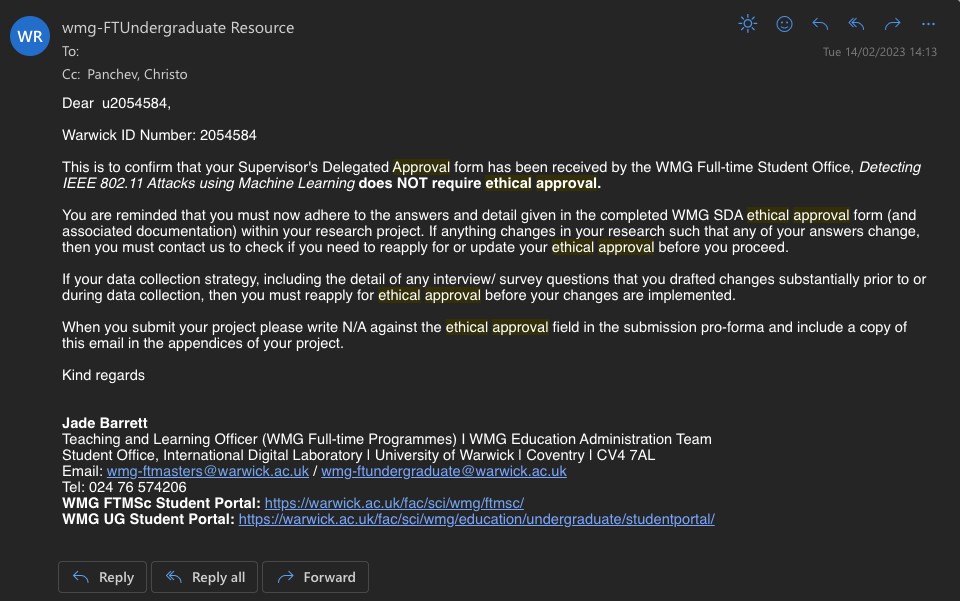
\includegraphics[width=\textwidth]{Appendices/Images/ethical_approval.png}
\end{center}

\begin{lstlisting}[language={}]
Dear 2054584,

Warwick ID Number: 2054584 

This is to confirm that your Supervisor's Delegated Approval form has been received by the WMG Full-time Student Office, Detecting IEEE 802.11 Attacks using Machine Learning does NOT require ethical approval.

You are reminded that you must now adhere to the answers and detail given in the completed WMG SDA ethical approval form (and associated documentation) within your research project. If anything changes in your research such that any of your answers change, then you must contact us to check if you need to reapply for or update your ethical approval before you proceed.

If your data collection strategy, including the detail of any interview/ survey questions that you drafted changes substantially prior to or during data collection, then you must reapply for ethical approval before your changes are implemented. 

When you submit your project please write N/A against the ethical approval field in the submission pro-forma and include a copy of this email in the appendices of your project.

Kind regards

Jade Barrett
\end{lstlisting}

\section{Dataset Manipulation}

\subsection{CSV Combiner Script}
\label{appx: CSV Combiner Script}
\begin{lstlisting}[language=bash, literate={-}{-}1]
#!/bin/bash

# Input Directory
input_dir="../Datasets"

cd "$input_dir"

# Set the output file name
output_file="../Datasets/combined/combined.csv"

# Check if the output file already exists and delete it
if [ -f "$output_file" ]; then
  rm "$output_file"
fi

echo "Combining files..."

# Loop through all the files
for file in $(ls *_reduced.csv | sort -V)
do
  # Check if the file exists
  if [ -f "$file" ]; then

    echo "Combining $file..."

    # For the first file, copy the header to the output file
    if [ ! -f "$output_file" ]; then
      head -n 1 "$file" > "$output_file"
    fi

    # Append all the rows except the header to the output file
    tail -n +2 "$file" >> "$output_file"
  fi
done

echo "Combining Finished"
\end{lstlisting}

\newpage
\subsection{Feature Extraction \& Reduction}
\label{appx: Feature Extraction}

\begin{lstlisting}[language=Python]
# Define the columns to extract
cols_to_use = [
	'frame.len','radiotap.dbm_antsignal','radiotap.length', 
	'wlan.duration','wlan_radio.duration','wlan_radio.signal_dbm', 
	'radiotap.present.tsft','wlan.fc.type','wlan.fc.subtype', 
	'wlan.fc.ds','wlan.fc.frag','wlan.fc.moredata',
	'wlan.fc.protected','wlan.fc.pwrmgt','wlan.fc.retry',
	'wlan_radio.phy','udp.length','ip.ttl',
	'arp','arp.proto.type','arp.hw.size',
	'arp.proto.size','arp.hw.type','arp.opcode',
  'tcp.analysis','tcp.analysis.retransmission','tcp.option_len',
  'tcp.checksum.status','tcp.flags.ack','tcp.flags.fin',
  'tcp.flags.push','tcp.flags.reset','tcp.flags.syn',
  'dns','dns.count.queries','dns.count.answers',
  'dns.resp.len','dns.resp.ttl','http.request.method',
  'http.response.code','http.content_type','ssh.message_code',
  'ssh.packet_length','nbns','nbss.length',
  'nbss.type','ldap','smb2.cmd',
  'smb.flags.response','smb.access.generic_read',
  'smb.access.generic_write','smb.access.generic_execute',
  'Label']

batch_size = 1000000

combined_df = pd.DataFrame()

# Iterate through the file in batches
for chunk in pd.read_csv('botnet_combined.csv', chunksize=batch_size, usecols=cols_to_use, low_memory=False):
    
    # Combine the processed chunk with previous chunks
    combined_df = pd.concat([combined_df, chunk])
\end{lstlisting}

\begin{lstlisting}[language=Python,linewidth=\textwidth]
# Drop all missing rows that contain only nan values
combined_df = combined_df.dropna(how='all')

# Drop all rows with missing values in Label Column
combined_df = combined_df.dropna(subset=['Label'])

# Fill NAs with zeros
# Change nan values to 0
combined_df = combined_df.fillna(0)
\end{lstlisting}

\newpage
\begin{lstlisting}
# Duplicate the dataframe
df = combined_df.copy()

# Regex to keep only the first value e.g 
# -100-100-10 becomes -100,   123-456-1 becomes 123, -10-2 becomes-10, 81-63-63 becomes 81
def seperated_values(x):
    x = str(x)
    match = re.match(r'^(-?\d+).*$', x)
    if match:
        return match.group(1)
    else:
        return x

# Go through all columns and change seperate values into just one value
for column in df.columns:
    df[column] = df[column].apply(seperated_values)
    print('Processing', column)
print('Done')

# Find Rows that contain values such as Oct-26, Oct-18, Feb-10 etc.. as these appear to be invalid and we will drop these rows.
regex = r"\b(?:\d{2}|(?:Jan|Feb|Mar|Apr|May|Jun|Jul|Aug|Sep|Oct|Nov|Dec))-(?:\d{2}|(?:Jan|Feb|Mar|Apr|May|Jun|Jul|Aug|Sep|Oct|Nov|Dec))\b"

# Use str.match method to apply the regex pattern to the column
mask = df['tcp.option_len'].astype(str).str.match(regex).fillna(False)
df = df[~mask]

mask = df['dns.resp.ttl'].astype(str).str.match(regex).fillna(False)
df = df[~mask]

mask = df['ip.ttl'].astype(str).str.match(regex).fillna(False)
df = df[~mask]

mask = df['smb2.cmd'].astype(str).str.match(regex).fillna(False)
df = df[~mask]

df.to_csv('Botnet_Reduced.csv', index=False)    

\end{lstlisting}

\newpage

\section{Conda Environments}
\label{appx: Conda_Env}

\subsection{Neural Networks - Apple Silicon}

\begin{lstlisting}
conda create -n nn-env python=3.9
conda activate nn-env
conda install -c apple tensorflow-deps
conda install -c conda-forge -y pandas jupyter
pip install tensorflow-macos==2.10
pip install numpy, matplotlib, scikit-learn, scipy, seaborn
\end{lstlisting}

\subsection{Classifiers}

\begin{lstlisting}
# Conda environment used for Random Forest, XGBoost and K-NN.

conda create -n ml-env python=3.9
conda activate ml-env
conda install -c conda-forge -y pandas jupyter
pip install numpy, matplotlib, scikit-learn, scipy, seaborn, xgboost
\end{lstlisting}

\newpage

\section{Data Preprocessing}
\label{appx:Data Processing}

\subsection{MinMax Scaling}
\label{appx:Scaling}

\begin{lstlisting}
# Define the scaler
scaler = MinMaxScaler()

# Fit the scaler to the following columns we define
scale_cols = [
        'frame.len',
        'radiotap.dbm_antsignal', 
        'radiotap.length', 
        'wlan.duration', 
        'wlan_radio.duration', 
        'wlan_radio.signal_dbm',
        'ip.ttl', 
        'udp.length', 
        'nbss.length',
        'dns.count.answers', 
        'dns.count.queries',
        'dns.resp.ttl',
        'ssh.packet_length']
        
# Fit the X_train and X_test
X_train[scale_cols] = scaler.fit_transform(X_train[scale_cols])
X_test[scale_cols] = scaler.transform(X_test[scale_cols])
\end{lstlisting}

\subsection{OHE Encoding}
\label{appx:OHE Encoding}
\begin{lstlisting}
cols_to_encode = [col for col in X_train.columns if col not in scale_cols]
X_all = pd.concat([X_train, X_test], axis=0)

X_all_ohe = pd.get_dummies(X_all, columns=cols_to_encode, drop_first=True, dtype=np.uint8)

# split back into train and test sets
X_train_ohe = X_all_ohe[:len(X_train)]
X_test_ohe = X_all_ohe[len(X_train):]
\end{lstlisting}

\newpage
\subsection{Label Encoding}
\label{appx:Label Encoding}
\begin{lstlisting}
    # Use Label Encoder to encode the target variable
le = LabelEncoder()

label_encoder = le.fit(y_train)
y_train_encoded = label_encoder.transform(y_train)
\end{lstlisting}

\subsection{Loading Dataset}
\label{appx:Loading Dataset}
\begin{lstlisting}
chunk_size = 1000000
dtype_opt = {
    'frame.len': 'int64',
    'radiotap.dbm_antsignal': 'int64',
    'radiotap.length': 'int64',
    'radiotap.present.tsft': 'int64',
    'wlan.duration': 'int64',
    'wlan.fc.ds': 'int64',
    'wlan.fc.frag': 'int64',
    'wlan.fc.moredata': 'int64',
    'wlan.fc.protected': 'int64',
    'wlan.fc.pwrmgt': 'int64',
    'wlan.fc.type': 'int64',
    'wlan.fc.retry': 'int64',
    'wlan.fc.subtype': 'int64',
    'wlan_radio.duration': 'int64',
    'wlan_radio.signal_dbm': 'int64',
    'wlan_radio.phy': 'int64',
    'arp': 'object',
    'arp.hw.type': 'object',
    'arp.proto.type': 'int64',
    'arp.hw.size': 'int64',
    'arp.proto.size': 'int64',
    'arp.opcode': 'int64',
    'ip.ttl': 'int64',
    'tcp.analysis': 'int64',
    'tcp.analysis.retransmission': 'int64',
    'tcp.checksum.status': 'int64',
    'tcp.flags.syn': 'int64',
    'tcp.flags.ack': 'int64',
    'tcp.flags.fin': 'int64',
    'tcp.flags.push': 'int64',
    'tcp.flags.reset': 'int64',
    'tcp.option_len': 'int64',
    'udp.length': 'int64',
    'nbns': 'object',
    'nbss.length': 'int64',
    'ldap': 'object',
    'smb2.cmd': 'int64',
    'dns': 'object',
    'dns.count.answers': 'int64',
    'dns.count.queries': 'int64',
    'dns.resp.ttl': 'int64',
    'http.content_type': 'object',
    'http.request.method': 'object',
    'http.response.code': 'int64',
    'ssh.message_code': 'int64',
    'ssh.packet_length': 'int64'
}

# Read the data
print('Reading X...')
X = pd.DataFrame()
for chunk in pd.read_csv('X.csv', chunksize=chunk_size, usecols=dtype_opt.keys(), dtype=dtype_opt, low_memory=False):
    X = pd.concat([X, chunk])

print('Reading y...')
y = pd.DataFrame()
for chunk in pd.read_csv('y.csv', chunksize=chunk_size, usecols=['Label'], dtype='object', low_memory=False):
   y = pd.concat([y, chunk])

# Split the data into training and testing sets
print('Splitting the data...')
X_train, X_test, y_train, y_test = train_test_split(X, y, test_size=0.30, random_state=1234, stratify=y)
\end{lstlisting}

\newpage
\section{Classifiers}
\label{appx: Classifiers}

\subsection{K-Nearest Neighbor (KNN)}
\begin{lstlisting}
# Use KNN
from sklearn.neighbors import KNeighborsClassifier

k=5

# Create KNN classifier
knn = KNeighborsClassifier(n_neighbors=k, n_jobs=-1)

# Fit the model
knn.fit(X_train_ohe, y_train_encoded)

# predict the test set
y_knn_pred = knn.predict(X_test_ohe)

from sklearn.metrics import classification_report, roc_auc_score

# Get the classification report
report = classification_report(y_test_encoded, y_knn_pred)

print('Classification Report:\n', report)

# Get the all the metrics for the multi class classification

print('Accuracy: ', accuracy_score(y_test_encoded, y_knn_pred))
print('Precision: ', precision_score(y_test_encoded, y_knn_pred, average='macro'))
print('Recall: ', recall_score(y_test_encoded, y_knn_pred, average='macro'))
print('F1 Score: ', f1_score(y_test_encoded, y_knn_pred, average='macro'))

# Get the confusion matrix for multi-class and plot it
confusion = confusion_matrix(y_test, y_rf_pred)
print('Confusion Matrix\n')
print(confusion)

# Plot the confusion matrix for multi-class classification using seaborn
labels = ['Normal', 'SSDP', 'Website Spoofing', 'Malware', 'Botnet', 'SSH', 'SQL Injection']

plt.figure(figsize=(8, 8))
sns.heatmap(confusion, annot=True, fmt='d', cmap='Blues', xticklabels=labels, yticklabels=labels)
plt.title('Confusion Matrix')
plt.xlabel('Predicted')
plt.ylabel('Actual')
plt.show()

plt.figure(figsize=(10, 10))
feat_importances = pd.Series(rf.feature_importances_, index=X_train_ohe.columns)
feat_importances.nlargest(20).plot(kind='barh')
plt.show()
\end{lstlisting}

\newpage

\subsection{Random Forest}
\label{appx:Random Forest}

\subsubsection{RF Model ID 0 - Raw Metrics}
\begin{lstlisting}[escapechar=!]
!\textbf{S-CV Results}!
Mean AUC = 99.99
Mean F1 = 99.66
Mean Precision = 99.66
Mean Recall = 99.67
Mean Accuracy = 99.67
Training Time: 7795 seconds

!\textbf{Final Test Results}!
Test AUC: 0.9999070506312879
Weighted Test F1: 0.996638797834701
Weighted Test Precision: 0.9966379719195173
Weighted Test Recall: 0.9967196932696956
Test Accuracy: 0.9967196932696956

!\textbf{Classification Report}!
                precision    recall  f1-score   support

      Botnet       0.95      0.77      0.85     17060
      Malware      0.89      0.82      0.86     39476
      Normal       1.00      1.00      1.00     457220
      SQL          0.93      0.86      0.89     789
      SSDP         1.00      1.00      1.00     1649955
      SSH          0.94      0.79      0.86     3565
      Spoofing     0.99      0.98      0.98     121533

    accuracy                           1.00   6404584
   macro avg       0.96      0.89      0.92   6404584
weighted avg       1.00      1.00      1.00   6404584

!\textbf{Confusion Matrix}!
[[  13082      17    3957       0       0       2       2]
 [     17   32454    6994       0       0      10       1]
 [    649    3821 4565771      51       2     161    1751]
 [      0       0     113     676       0       0       0]
 [      0       0       2       0 1649953       0       0]
 [      5      20     707       0       0    2833       0]
 [      4       0    2723       0       0       0  118806]]
\end{lstlisting}

\begin{center}
	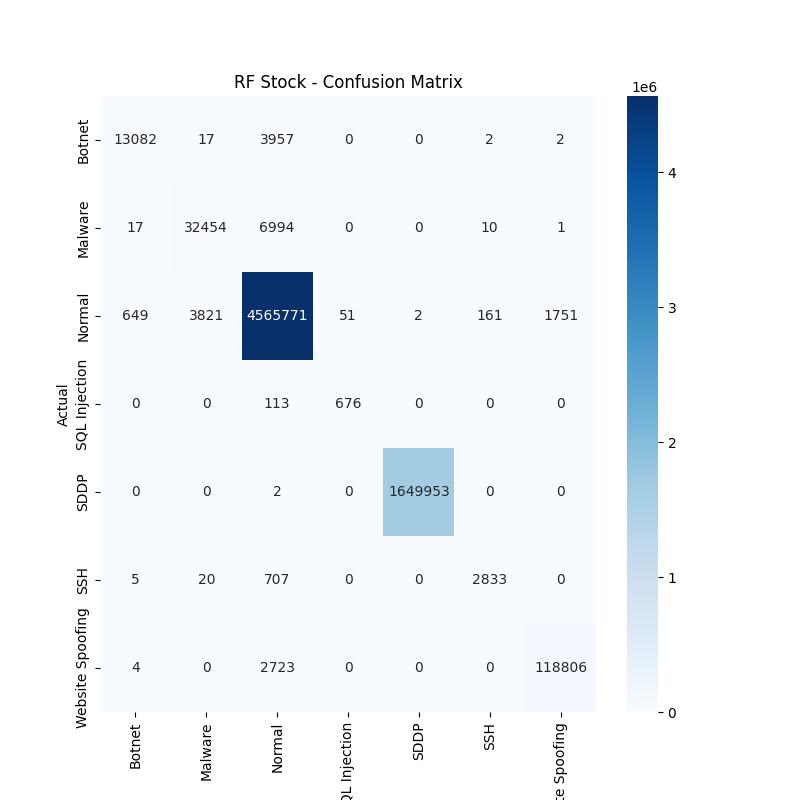
\includegraphics[scale=0.8]{Appendices/Images/RF/Model0/rf_stock_cm.png}
	\captionof*{figure}{RF Model 0 - Confusion Matrix}
\end{center}


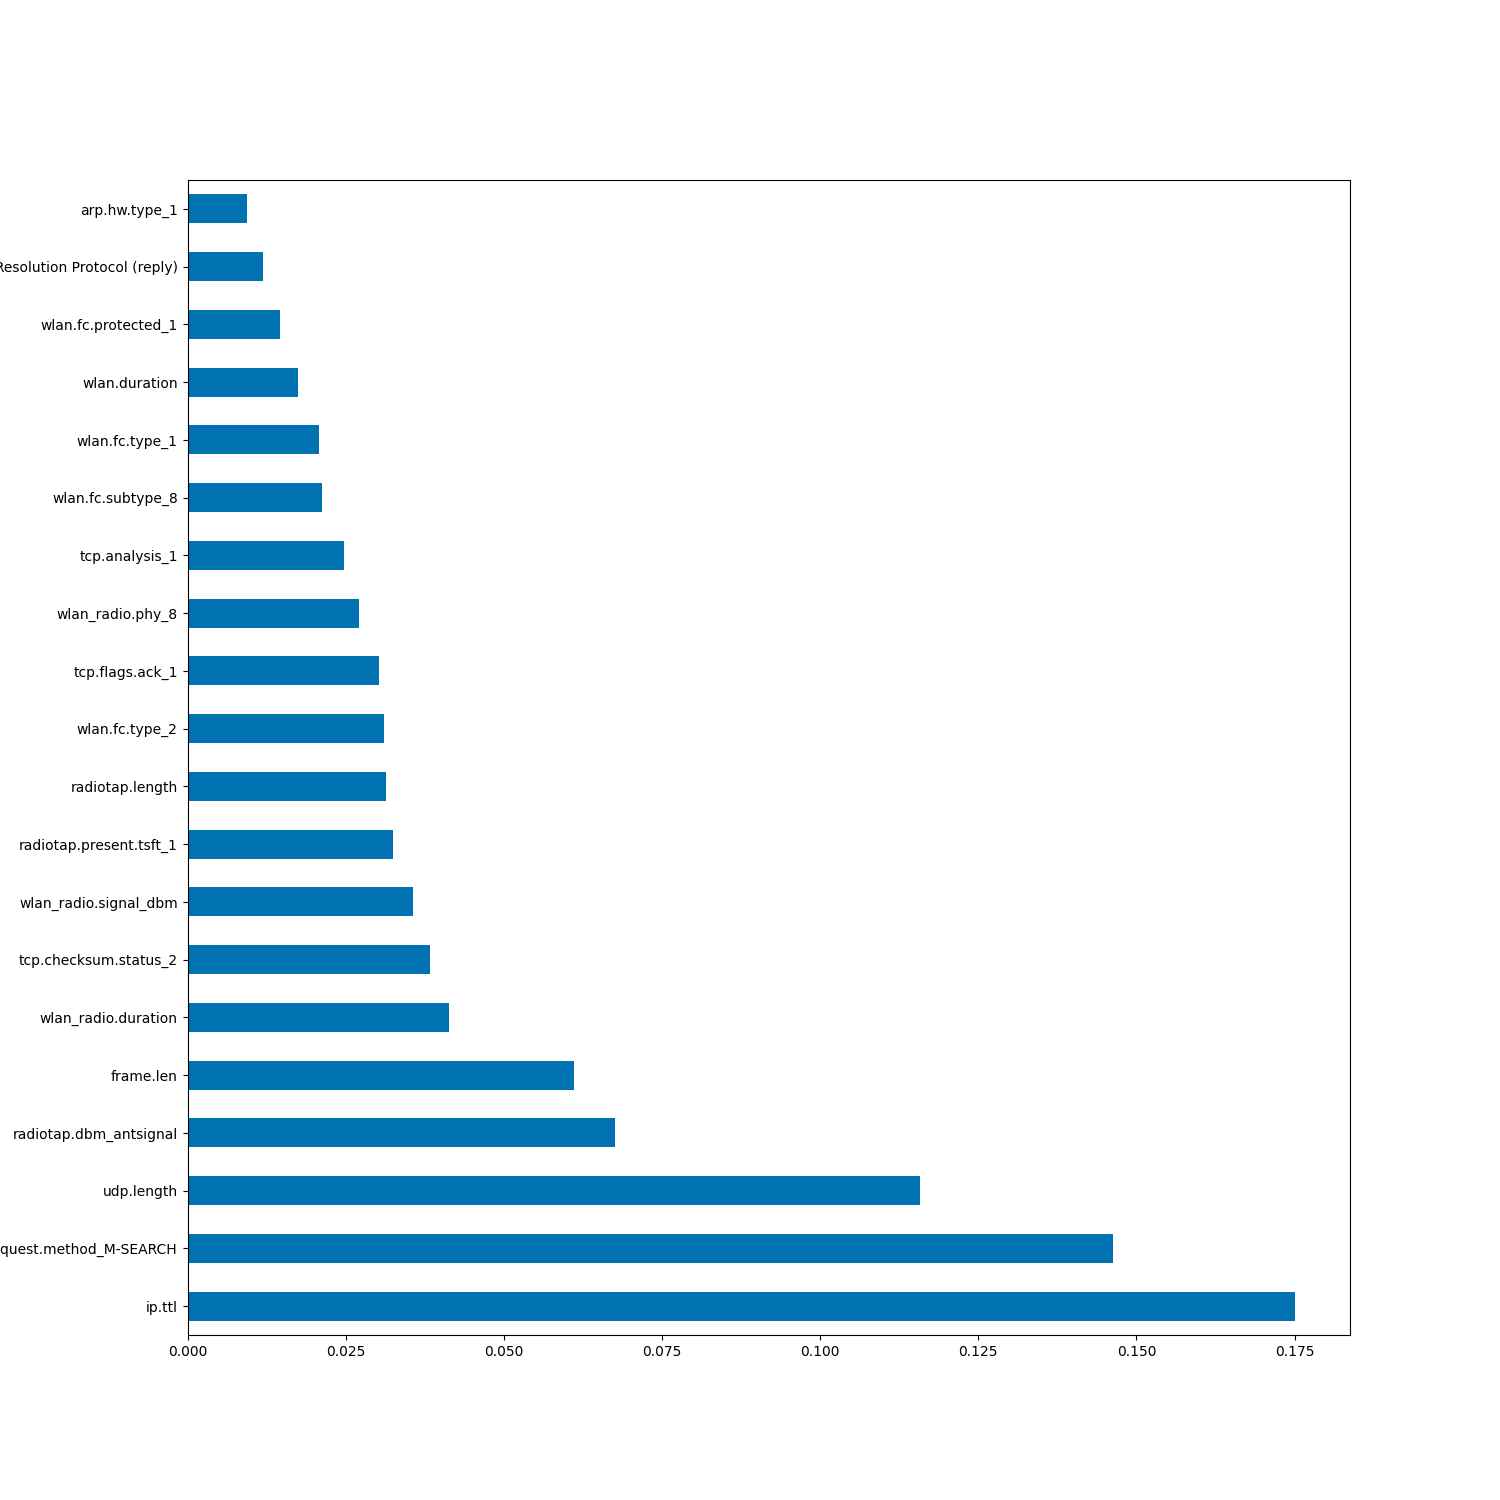
\includegraphics[width=\textwidth]{Appendices/Images/RF/Model0/rf_stock_feature_imp.png}

\newpage
\subsubsection{RF Model ID 1 - Raw Metrics}
\begin{lstlisting}[escapechar=!]
!\textbf{S-CV Results}!
Mean AUC = 99.99
Mean F1 = 99.66
Mean Precision = 99.66
Mean Recall = 99.67
Mean Accuracy = 99.67
Training Time 7794.549654006958 seconds

!\textbf{Final Test Results}!
Test AUC: 0.9999070506312879
Weighted Test F1: 0.996638797834701
Weighted Test Precision: 0.9966379719195173
Weighted Test Recall: 0.9967196932696956
Test Accuracy: 0.9967196932696956

!\textbf{Classification Report}!
			          precision    recall  f1-score   support

      Botnet       0.95      0.77      0.85     17060
     Malware       0.89      0.82      0.86     39476
      Normal       1.00      1.00      1.00   4572206
         SQL       0.93      0.86      0.89       789
        SSDP       1.00      1.00      1.00   1649955
         SSH       0.94      0.79      0.86      3565
WebsiteSpoof       0.99      0.98      0.98    121533

    accuracy                           1.00   6404584
   macro avg       0.96      0.89      0.92   6404584
weighted avg       1.00      1.00      1.00   6404584
    
!\textbf{Confusion Matrix}!    
[[  13082      17    3957       0       0       2       2]
 [     17   32454    6994       0       0      10       1]
 [    649    3821 4565771      51       2     161    1751]
 [      0       0     113     676       0       0       0]
 [      0       0       2       0 1649953       0       0]
 [      5      20     707       0       0    2833       0]
 [      4       0    2723       0       0       0  118806]]
\end{lstlisting}

\begin{center}
	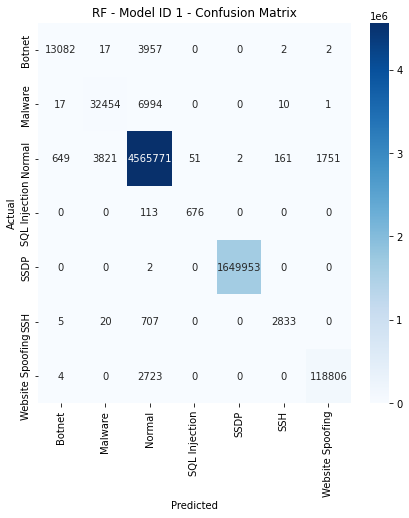
\includegraphics[width=\textwidth]{Appendices/Images/RF/Model1/RF_Model1_CM.png}
	\captionof*{figure}{RF Model 1 - Confusion Matrix}
	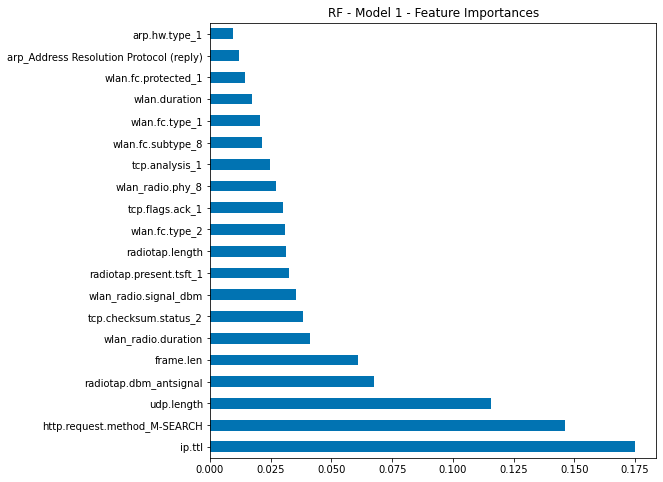
\includegraphics[width=\textwidth]{Appendices/Images/RF/Model1/RF_Model1_FI.png}
	\captionof*{figure}{RF Model 1 - Feature Importance}
\end{center}

\newpage
\subsubsection{RF Model ID 2 - Raw Metrics}
\begin{lstlisting}[escapechar=!]
!\textbf{Final Test Results}!
Test AUC:  0.9999070506308619
Weighted Test Precision:  0.9966379719195173
Weighted Test Recall:  0.9967196932696956
Weighted Test F1:  0.996638797834701
Test Accuracy:  0.9967196932696956

!\textbf{Classification Report}!
				          precision    recall  f1-score   support

          Botnet       0.95      0.77      0.85     17060
         Malware       0.89      0.82      0.86     39476
          Normal       1.00      1.00      1.00   4572206
   SQL_Injection       0.93      0.86      0.89       789
            SSDP       1.00      1.00      1.00   1649955
             SSH       0.94      0.79      0.86      3565
Website_spoofing       0.99      0.98      0.98    121533

        accuracy                           1.00   6404584
       macro avg       0.96      0.89      0.92   6404584
    weighted avg       1.00      1.00      1.00   6404584
    
!\textbf{Confusion Matrix}!    
[[  13082      17    3957       0       0       2       2]
 [     17   32454    6994       0       0      10       1]
 [    649    3821 4565771      51       2     161    1751]
 [      0       0     113     676       0       0       0]
 [      0       0       2       0 1649953       0       0]
 [      5      20     707       0       0    2833       0]
 [      4       0    2723       0       0       0  118806]]
\end{lstlisting}
\begin{center}
	\centering
	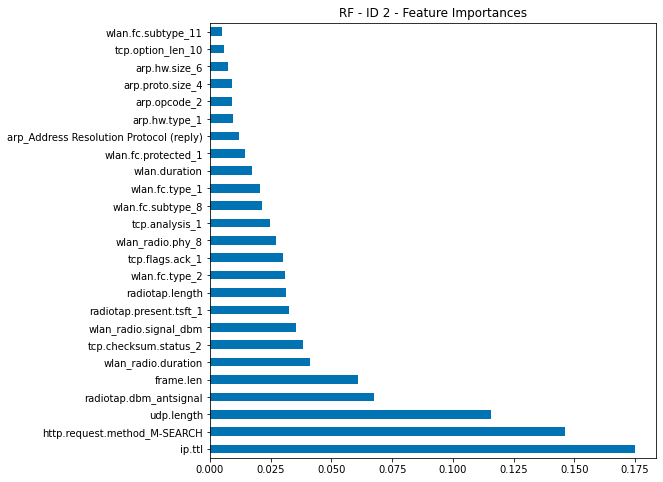
\includegraphics[width=\textwidth]{Appendices/Images/RF/Model2/RF_Model2_FI.png}
	\captionof*{figure}{RF Model 2 - Feature Importance}
\end{center}


\newpage
\subsubsection{RF Model ID 3 - Raw Metrics}
\begin{lstlisting}[escapechar=!]
!\textbf{S-CV Results}!
Mean AUC = 0.9999
Mean F1 = 0.9966
Mean Precision = 0.9966
Mean Recall = 0.9967
Mean Accuracy = 0.9967
Training Time 56042.87267756462  seconds

!\textbf{Final Test Results}!
Test AUC:  0.9999070506308619
Weighted Test F1:  0.996638797834701
Weighted Test Precision:  0.9966379719195173
Weighted Test Recall:  0.9967196932696956
Test Accuracy:  0.9967196932696956

!\textbf{Classification Report}!
				          precision    recall  f1-score   support
				  
          Botnet       0.95      0.77      0.85     17060
         Malware       0.89      0.82      0.86     39476
          Normal       1.00      1.00      1.00   4572206
   SQL_Injection       0.93      0.86      0.89       789
            SSDP       1.00      1.00      1.00   1649955
             SSH       0.94      0.79      0.86      3565
Website_spoofing       0.99      0.98      0.98    121533

        accuracy                           1.00   6404584
       macro avg       0.96      0.89      0.92   6404584
    weighted avg       1.00      1.00      1.00   6404584
    
    
!\textbf{Confusion Matrix}!

[[  13082      17    3957       0       0       2       2]
 [     17   32454    6994       0       0      10       1]
 [    649    3821 4565771      51       2     161    1751]
 [      0       0     113     676       0       0       0]
 [      0       0       2       0 1649953       0       0]
 [      5      20     707       0       0    2833       0]
 [      4       0    2723       0       0       0  118806]]
\end{lstlisting}
\begin{center}
	\centering
	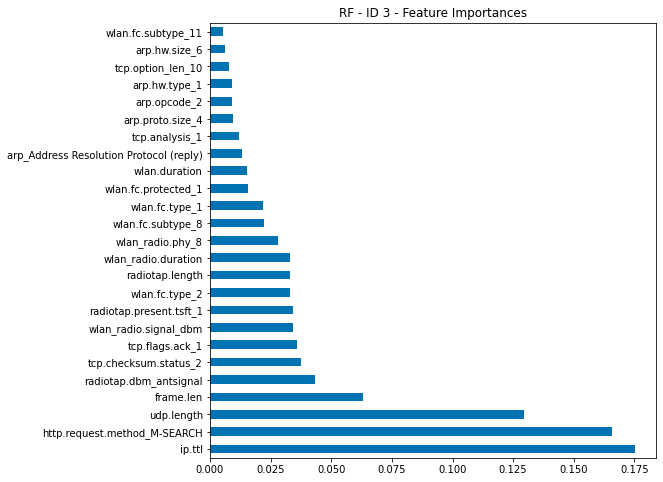
\includegraphics[width=\textwidth]{Appendices/Images/RF/Model3/RF_Model3_FI.png}
	\captionof*{figure}{RF Model 3 - Feature Importance}
\end{center}

\newpage
\subsubsection{RF Model ID 4 - Raw Metrics}
\begin{lstlisting}[escapechar=!]
!\textbf{S-CV Results}!
Mean AUC = 99.95
Mean F1 = 95.23
Mean Precision = 98.50
Mean Recall = 92.96
Mean Accuracy = 92.96
Training Time = 10147 seconds

!\textbf{Final Test Results}!
Test AUC: 0.9994792868436975
Weighted Test Precision: 0.984757273176817
Weighted Test Recall: 0.925409987596384
Weighted Test F1: 0.9496738038716113
Test Accuracy: 0.925409987596384

!\textbf{Classification Report}!

                  precision    recall  f1-score   support

          Botnet       0.14      0.96      0.24     17060
         Malware       0.22      0.97      0.36     39476
          Normal       1.00      0.90      0.95   4572206
   SQL_Injection       0.01      0.99      0.02       789
            SSDP       1.00      1.00      1.00   1649955
             SSH       0.04      0.99      0.08      3565
Website_spoofing       0.61      0.98      0.75    121533
           
        accuracy                           0.93   6404584
       macro avg       0.43      0.97      0.48   6404584
    weighted avg       0.98      0.93      0.95   6404584
    
    
!\textbf{Confusion Matrix}!

[[  16326      90      30      91       0     504      19]
 [     76   38392      13     170       0     824       1]
 [ 102163  135709 4098890   76381       2   83351   75710]
 [      0       0       1     785       0       3       0]
 [      0       0      10       0 1649945       0       0]
 [      6      15       4      16       0    3523       1]
 [    282    1145     484     262       0     355  119005]]
\end{lstlisting}
\begin{center}
	\centering
	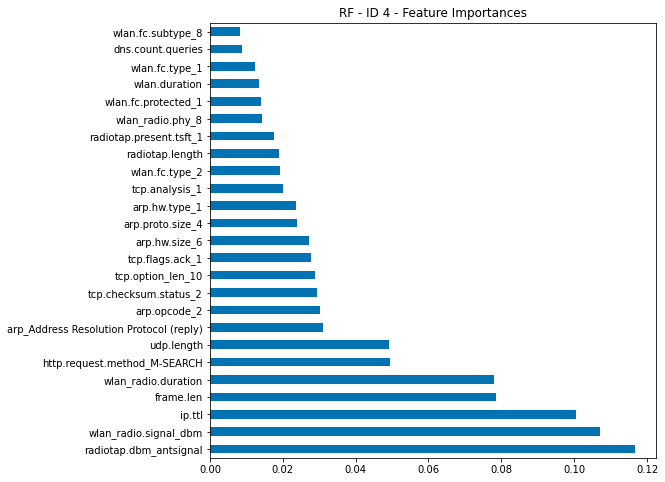
\includegraphics[width=\textwidth]{Appendices/Images/RF/Model4/RF_Model4_FI.png}
\end{center}

\newpage
\subsubsection{RF Model ID 5 - Raw Metrics}
\begin{lstlisting}[escapechar=!]
!\textbf{S-CV Results}!
Mean AUC = 0.9987
Mean F1 = 0.9153
Mean Precision = 0.9842
Mean Recall = 0.8665
Mean Accuracy = 0.8665
Training Time 4632.155310869217 seconds

!\textbf{Final Test Results}!
Test AUC: 0.998635554230961
Weighted Test Precision: 0.9848384599880898
Weighted Test Recall: 0.8600619493787575
Weighted Test F1: 0.9116563847511311
Test Accuracy: 0.8600619493787575

!\textbf{Classification Report}!

			          precision    recall  f1-score   support

      Botnet       0.06      0.94      0.12     17060
     Malware       0.10      0.90      0.19     39476
      Normal       1.00      0.81      0.89   4572206
         SQL       0.01      0.99      0.01       789
        SSDP       0.99      1.00      1.00   1649955
         SSH       0.02      0.99      0.04      3565
    WebSpoof       0.76      0.92      0.83    121533

    accuracy                           0.86   6404584
   macro avg       0.42      0.94      0.44   6404584
weighted avg       0.98      0.86      0.91   6404584
    
    
!\textbf{Confusion Matrix}!

[[  16064     141      26     133       0     693       3]
 [     72   35584     121     125       0    3572       2]
 [ 240322  301805 3690025  138640   11696  154013   35705]
 [      0       0       0     783       0       5       1]
 [      0       0       9       0 1649946       0       0]
 [      6       1       0      12       0    3546       0]
 [   4970    1711     301    1392       0     768  112391]]
\end{lstlisting}

\begin{center}
	\centering
	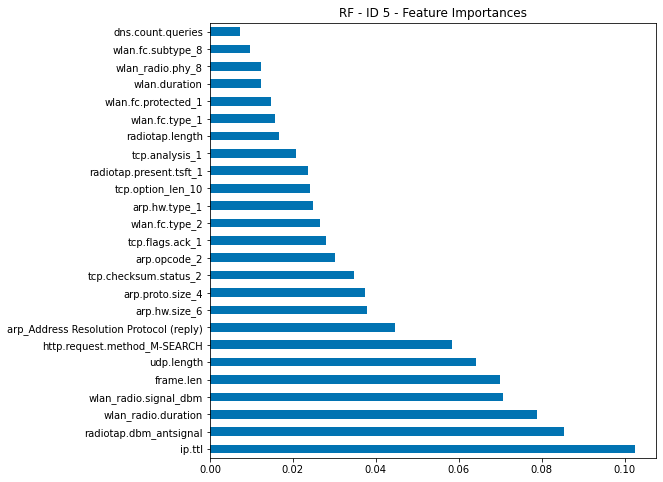
\includegraphics[width=\textwidth]{Appendices/Images/RF/Model5/RF_Model5_FI.png}
	\captionof*{figure}{RF Model 5 - Feature Importance}
\end{center}


% XGBOOOOOOOOOST

\newpage
\subsection{XGBoost}
\label{appx:XGBoost}


\subsubsection{XGBoost Model 0 - Raw Metrics}
\begin{lstlisting}[escapechar=!]

!\textbf{Final Test Results}!
Test AUC: 0.9999
Weighted F1: 0.9963
Weighted Precision: 0.9964
Weighted Recall: 0.9964
Test Accuracy: 0.9964

!\textbf{Classification Report}!
			          precision    recall  f1-score   support

      Botnet       0.96      0.74      0.83     10236
     Malware       0.86      0.85      0.86     23686
      Normal       1.00      1.00      1.00   2743324
         SQL       0.95      0.87      0.91       473
        SSDP       1.00      1.00      1.00    989973
         SSH       0.90      0.77      0.83      2139
    WebSpoof       0.99      0.97      0.98     72920

    accuracy                           1.00   3842751
   macro avg       0.95      0.88      0.91   3842751
weighted avg       1.00      1.00      1.00   3842751
    
!\textbf{Confusion Matrix}!    
[[   7538      29    2664       0       0       2       3]
 [     19   20191    3471       0       0       5       0]
 [    273    3282 2738552      20       1     185    1011]
 [      0       0      63     410       0       0       0]
 [      0       0       1       0  989972       0       0]
 [      4      11     484       0       0    1640       0]
 [      3       1    2319       0       0       0   70597]]

\end{lstlisting}

\begin{center}
	\centering
	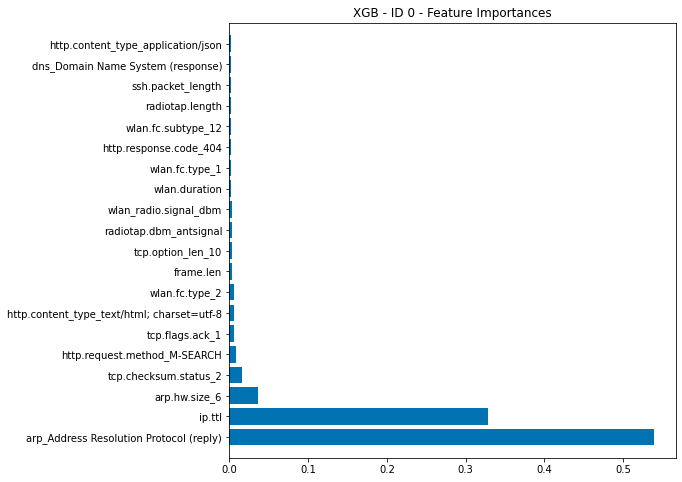
\includegraphics[width=\textwidth]{Appendices/Images/XGB/Model0/XGB_Model0_FI.png}
	\captionof*{figure}{XGBoost Model 0 - Feature Importance}
\end{center}


\subsubsection{XGBoost Model 1 - Raw Metrics}
\begin{lstlisting}[escapechar=!]
!\textbf{S-CV Results}!


!\textbf{Final Test Results}!
Test AUC: 0.9999
Weighted Test F1: 0.9964
Weighted Test Precision: 0.9965
Weighted Test Recall: 0.9965
Test Accuracy: 0.9965

!\textbf{Classification Report}!
			          precision    recall  f1-score   support

      Botnet       0.96      0.75      0.84     13648
     Malware       0.86      0.86      0.86     31581
      Normal       1.00      1.00      1.00   3657765
         SQL       0.94      0.84      0.89       631
        SSDP       1.00      1.00      1.00   1319964
         SSH       0.95      0.76      0.84      2852
    WebSpoof       0.99      0.97      0.98     97226

    accuracy                           1.00   5123667
   macro avg       0.96      0.88      0.91   5123667
weighted avg       1.00      1.00      1.00   5123667
    
!\textbf{Confusion Matrix}!    
[[  10250      10    3382       0       0       1       5]
 [     40   27004    4533       0       0       3       1]
 [    406    4444 3651488      36       1     108    1282]
 [      0       0     101     530       0       0       0]
 [      0       0       6       0 1319958       0       0]
 [      3      19     670       0       0    2160       0]
 [      0       8    2841       0       0       0   94377]]

\end{lstlisting}

\begin{center}
	\centering
	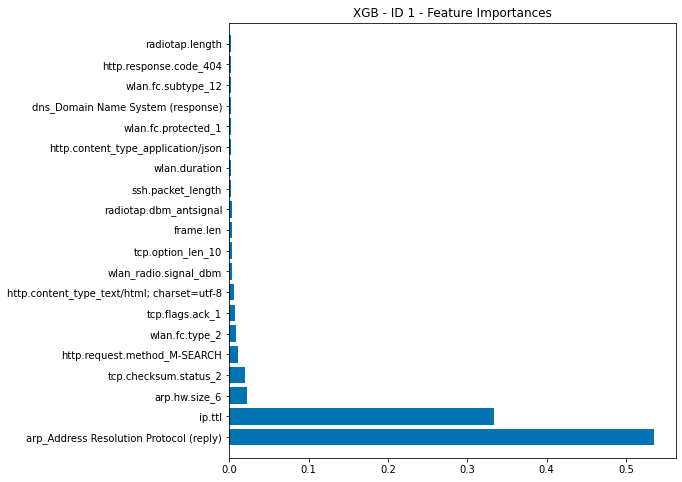
\includegraphics[width=\textwidth]{Appendices/Images/XGB/Model1/XGB_Model1_FI.png}
	\captionof*{figure}{XGBoost Model 1 - Feature Importance}
\end{center}

\subsubsection{XGBoost Model 2 - Raw Metrics}
\begin{lstlisting}[escapechar=!]

!\textbf{Final Test Results}!
Test AUC: 0.9999
Weighted Test F1: 0.9964
Weighted Test Precision: 0.9964
Weighted Test Recall: 0.9964
Test Accuracy: 0.9964

!\textbf{Classification Report}!
			     precision    recall  f1-score   support

      Botnet       0.97      0.74      0.84     13648
     Malware       0.85      0.86      0.86     31581
      Normal       1.00      1.00      1.00   3657765
         SQL       0.93      0.84      0.88       631
        SSDP       1.00      1.00      1.00   1319964
         SSH       0.91      0.74      0.82      2852
    WebSpoof       0.99      0.97      0.98     97226

    accuracy                           1.00   5123667
   macro avg       0.95      0.88      0.91   5123667
weighted avg       1.00      1.00      1.00   5123667
    
!\textbf{Confusion Matrix}!    
[[  10094      20    3528       0       0       2       4]
 [     34   27180    4365       0       0       2       0]
 [    331    4611 3651281      38       1     203    1300]
 [      0       0     103     528       0       0       0]
 [      0       0       6       0 1319958       0       0]
 [      1      19     714       0       0    2118       0]
 [      0       4    2950       0       0       0   94272]]

\end{lstlisting}
\begin{center}
	\centering
	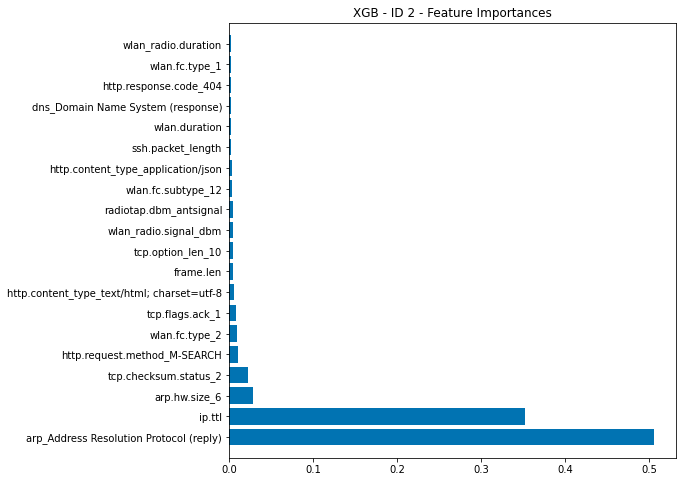
\includegraphics[width=\textwidth]{Appendices/Images/XGB/Model2/XGB_Model2_FI.png}
	\captionof*{figure}{XGBoost Model 2 - Feature Importance}
\end{center}

\subsubsection{XGBoost Model 3 - Raw Metrics}
\begin{lstlisting}[escapechar=!]
!\textbf{Final Test Results}!
Test AUC: 0.9999
Weighted Test F1: 0.9964
Weighted Test Precision: 0.9964
Weighted Test Recall: 0.9964
Test Accuracy: 0.9964

!\textbf{Classification Report}!
			           precision    recall  f1-score   support

      Botnet       0.96      0.74      0.84     13648
     Malware       0.85      0.86      0.86     31581
      Normal       1.00      1.00      1.00   3657765
         SQL       0.94      0.85      0.89       631
        SSDP       1.00      1.00      1.00   1319964
         SSH       0.92      0.74      0.82      2852
    WebSpoof       0.99      0.97      0.98     97226

    accuracy                           1.00   5123667
   macro avg       0.95      0.88      0.91   5123667
weighted avg       1.00      1.00      1.00   5123667
    
!\textbf{Confusion Matrix}!    
[[  10133       9    3499       0       0       1       6]
 [     36   27171    4370       0       0       3       1]
 [    350    4621 3651253      35       1     193    1312]
 [      0       0      93     538       0       0       0]
 [      0       0       6       0 1319958       0       0]
 [      4      19     705       0       0    2124       0]
 [      0      10    2921       0       0       0   94295]]

\end{lstlisting}
\begin{center}
	\centering
	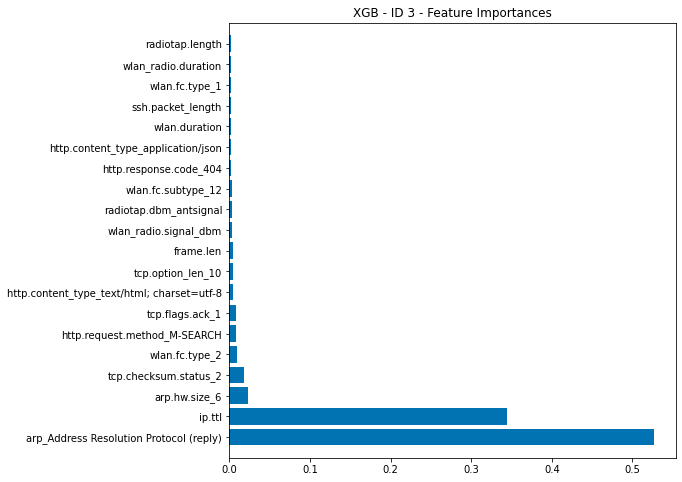
\includegraphics[width=\textwidth]{Appendices/Images/XGB/Model3/XGB_Model3_FI.png}
	\captionof*{figure}{XGBoost Model 3 - Feature Importance}
\end{center}


\subsubsection{XGBoost Model 4 - Raw Metrics}
\begin{lstlisting}[escapechar=!]
!\textbf{GridSearchCV Results}!
Searching took 101767.660586 seconds
{'learning_rate': 0.2, 'max_depth': 5, 'n_estimators': 300}
0.9964800321988857
\end{lstlisting}

\subsubsection{XGBoost Model 5 - Raw Metrics}
\begin{lstlisting}[escapechar=!]

!\textbf{Final Test Results}!
Test AUC: 0.9999
Weighted Test F1: 0.9964
Weighted Test Precision: 0.9965
Weighted Test Recall: 0.9965
Test Accuracy: 0.9965

!\textbf{Classification Report}!
			     precision    recall  f1-score   support

      Botnet       0.96      0.75      0.84     13648
     Malware       0.85      0.86      0.86     31581
      Normal       1.00      1.00      1.00   3657765
         SQL       0.93      0.87      0.90       631
        SSDP       1.00      1.00      1.00   1319964
         SSH       0.91      0.76      0.83      2852
    WebSpoof       0.99      0.97      0.98     97226

    accuracy                           1.00   5123667
   macro avg       0.95      0.89      0.91   5123667
weighted avg       1.00      1.00      1.00   5123667
    
!\textbf{Confusion Matrix}!    
[[  10251      15    3378       0       0       2       2]
 [     35   27290    4239       0       0       5      12]
 [    424    4709 3651040      42       1     213    1336]
 [      0       0      84     547       0       0       0]
 [      0       0       6       0 1319958       0       0]
 [      0      19     671       0       0    2162       0]
 [      0       6    2832       0       0       0   94388]]

\end{lstlisting}

\begin{center}
	\centering
	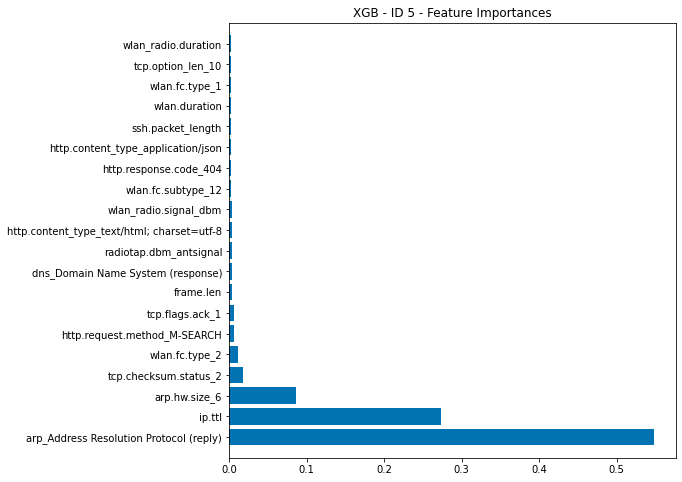
\includegraphics[width=\textwidth]{Appendices/Images/XGB/Model5/XGB_Model5_FI.png}
	\captionof*{figure}{XGBoost Model 5 - Feature Importance}
\end{center}

\subsubsection{XGBoost Model 6 - Raw Metrics}
\begin{lstlisting}[escapechar=!]

!\textbf{Final Test Results}!
Test AUC: 99.99
Weighted Test F1: 99.65
Weighted Test Precision: 99.65
Weighted Test Recall: 99.65
Test Accuracy: 99.65

!\textbf{Classification Report}!
			             precision    recall  f1-score   support

      Botnet       0.96      0.74      0.84     17060
     Malware       0.86      0.85      0.86     39476
      Normal       1.00      1.00      1.00   3657765
         SQL       0.93      0.88      0.90       789
        SSDP       1.00      1.00      1.00   1649955
         SSH       0.95      0.79      0.86      3565
    WebSpoof       0.99      0.97      0.98    121533

    accuracy                           1.00   6404584
   macro avg       0.95      0.89      0.92   6404584
weighted avg       1.00      1.00      1.00   6404584
    
!\textbf{Confusion Matrix}!    
[[  12703      31    4320       0       0       2       4]
 [     17   33596    5857       0       0       6       0]
 [    539    5289 4564546      56       0     144    1632]
 [      0       0      91     698       0       0       0]
 [      0       0       0       0 1649955       0       0]
 [      5      15     745       0       0    2800       0]
 [      1       4    3344       0       0       0  118184]]

\end{lstlisting}
\begin{center}
	\centering
	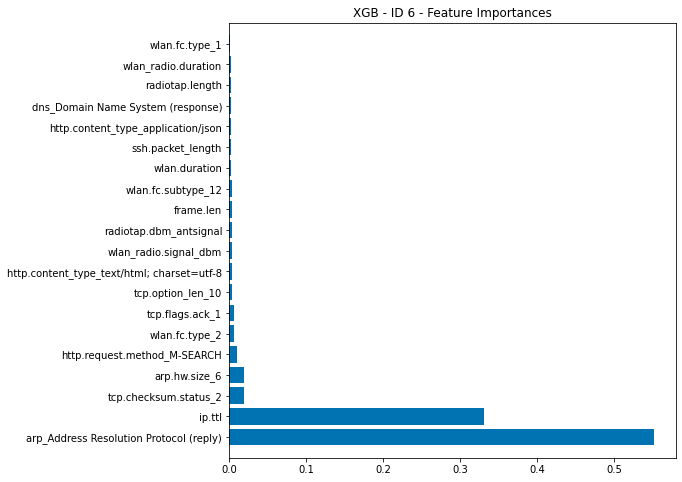
\includegraphics[width=\textwidth]{Appendices/Images/XGB/Model6/XGB_Model6_FI.png}
	\captionof*{figure}{XGBoost Model 6 - Feature Importance}
\end{center}

\subsubsection{XGBoost Model 7 - Raw Metrics}
\begin{lstlisting}[escapechar=!]

!\textbf{Final Test Results}!
Test AUC: 99.99
Weighted Test F1: 99.65
Weighted Test Precision: 99.65
Weighted Test Recall: 99.65
Test Accuracy: 99.65

!\textbf{Classification Report}!
			       precision    recall  f1-score   support

      Botnet       0.96      0.74      0.84     17060
     Malware       0.86      0.86      0.86     39476
      Normal       1.00      1.00      1.00   3657765
         SQL       0.93      0.89      0.91       789
        SSDP       1.00      1.00      1.00   1649955
         SSH       0.92      0.78      0.84      3565
    WebSpoof       0.99      0.97      0.98    121533

    accuracy                           1.00   6404584
   macro avg       0.95      0.89      0.92   6404584
weighted avg       1.00      1.00      1.00   6404584
    
!\textbf{Confusion Matrix}!    
[[  12640      28    4387       0       0       2       3]
 [     17   34017    5434       0       0       8       0]
 [    546    5657 4564062      51       3     244    1643]
 [      0       0      87     702       0       0       0]
 [      0       0       0       0 1649955       0       0]
 [      3      14     760       0       0    2788       0]
 [      1      11    3341       0       0       0  118180]]

\end{lstlisting}
\begin{center}
	\centering
	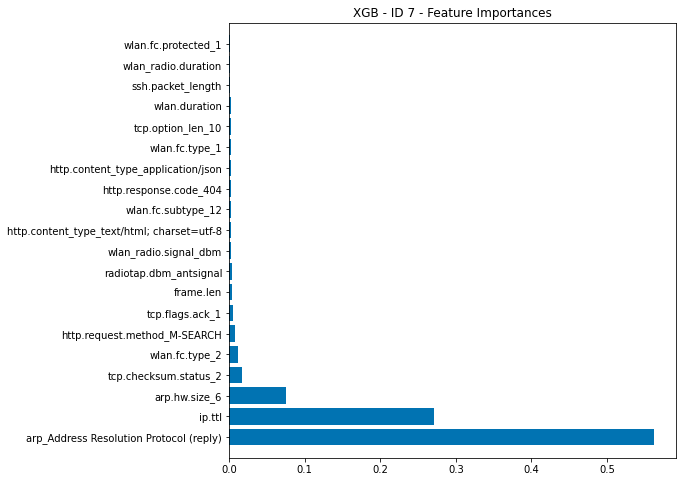
\includegraphics[width=\textwidth]{Appendices/Images/XGB/Model7/XGB_Model7_FI.png}
	\captionof*{figure}{XGBoost Model 7 - Feature Importance}
\end{center}

\subsubsection{XGBoost Model 8 - Raw Metrics}
\begin{lstlisting}[escapechar=!]
!\textbf{S-CV Results}!


!\textbf{Final Test Results}!
Test AUC: 99.99
Weighted Test F1: 99.65
Weighted Test Precision: 99.65
Weighted Test Recall: 99.65
Test Accuracy: 99.65

!\textbf{Classification Report}!
					 precision    recall  f1-score   support

        Botnet       0.96      0.74      0.84     17060
       Malware       0.86      0.86      0.86     39476
        Normal       1.00      1.00      1.00   4572206
           SQL       0.93      0.89      0.91       789
          SSDP       1.00      1.00      1.00   1649955
           SSH       0.92      0.78      0.85      3565
      WebSpoof       0.99      0.97      0.98    121533

     accuracy                            1.00   6404584
    macro avg        0.95      0.89      0.92   6404584
 weighted avg        1.00      1.00      1.00   6404584
    
!\textbf{Confusion Matrix}!    
[[  12631      28    4396       0       0       2       3]
 [     17   34025    5426       0       0       8       0]
 [    539    5665 4564060      51       3     242    1646]
 [      0       0      89     700       0       0       0]
 [      0       0       0       0 1649955       0       0]
 [      3      14     755       0       0    2793       0]
 [      1      11    3308       0       0       0  118213]]

\end{lstlisting}

\subsubsection{XGBoost Model 9 - Raw Metrics}
\begin{lstlisting}[escapechar=!]
!\textbf{RandomisedGridSearchResults}!
Time taken for CV: 150508.66 seconds
Best parameters found:  
{'subsample': 0.9, 
 'n_estimators': 200, 
 'min_child_weight': 3, 
 'max_depth': 9, 
 'learning_rate': 0.3, 
 'gamma': 0, 
 'colsample_bytree': 0.7
}
\end{lstlisting}

\subsubsection{XGBoost Model 10 - Raw Metrics}
\begin{lstlisting}[escapechar=!]
!\textbf{S-CV Results}!
Average AUC: 0.9999621491771731 
Average F1-score: 0.9965027851331616
Average Precision: 0.9965087377065057
Average Recall: 0.9965808417525853
Average Accuracy: 0.9965808417525853

!\textbf{Final Test Results}!
Test ROC AUC:  99.98872586203336
Weighted Test F1:  99.65319267148135
Weighted Test Precision:  99.65352146874279
Weighted Test Recall:  99.66211700869252
Test Accuracy:  99.66211700869252

!\textbf{Classification Report}!
				       precision    recall  f1-score   support

      Botnet       0.96      0.75      0.84     17060
     Malware       0.89      0.82      0.85     39476
      Normal       1.00      1.00      1.00   4572206
         SQL       0.94      0.89      0.91       789
        SSDP       1.00      1.00      1.00   1649955
         SSH       0.92      0.78      0.85      3565
    WebSpoof       0.99      0.97      0.98    121533

    accuracy                           1.00   6404584
   macro avg       0.96      0.89      0.92   6404584
weighted avg       1.00      1.00      1.00   6404584
    
!\textbf{Confusion Matrix}!    
[[  12852      17    4183       0       0       3       5]
 [     18   32315    7132       0       0       8       3]
 [    580    3781 4565841      47       3     241    1713]
 [      0       0      89     700       0       0       0]
 [      0       0       0       0 1649955       0       0]
 [      6      15     749       0       0    2794       1]
 [      1       4    3041       0       0       0  118487]]

\end{lstlisting}
\begin{center}
	\centering
	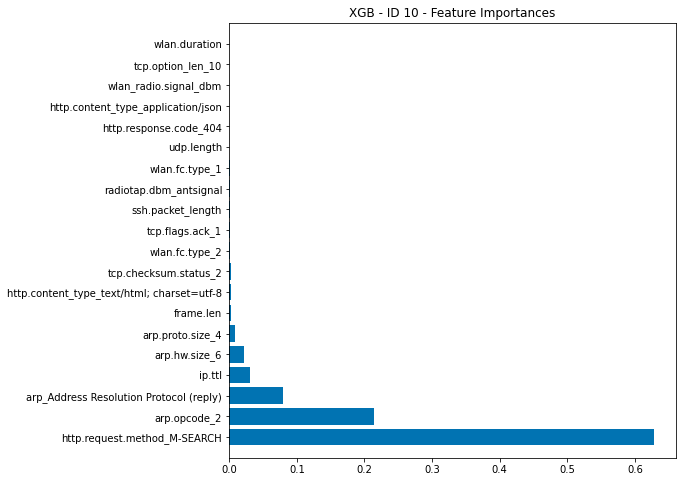
\includegraphics[width=\textwidth]{Appendices/Images/XGB/Model10/XGB_Model10_FI.png}
	\captionof*{figure}{XGBoost Model 10 - Feature Importance}
\end{center}


\subsubsection{XGBoost Model 11 - Raw Metrics}
\begin{lstlisting}[escapechar=!]
!\textbf{S-CV Results}!
Average AUC: 99.99578159885314
Average F1-score: 99.64055055296684
Average Precision: 99.6431971824485
Average Recall: 99.6459656226469
Average Accuracy: 99.6459656226469
Training Time: 1450.04 seconds

!\textbf{Final Test Results}!
Test AUC:  99.98690081277596
Weighted Test F1:  99.64724140077732
Weighted Test Precision:  99.64992342160565
Weighted Test Recall:  99.65274871873021
Test Accuracy:  99.65274871873021

!\textbf{Classification Report}!
				       precision    recall  f1-score   support

      Botnet       0.96      0.74      0.84     17060
     Malware       0.86      0.86      0.86     39476
      Normal       1.00      1.00      1.00   4572206
         SQL       0.93      0.89      0.91       789
        SSDP       1.00      1.00      1.00   1649955
         SSH       0.92      0.78      0.84      3565
    WebSpoof       0.99      0.97      0.98    121533

    accuracy                           1.00   6404584
   macro avg       0.95      0.89      0.92   6404584
weighted avg       1.00      1.00      1.00   6404584
    
!\textbf{Confusion Matrix}!    
[[  12640      28    4387       0       0       2       3]
 [     17   34017    5434       0       0       8       0]
 [    546    5657 4564062      51       3     244    1643]
 [      0       0      87     702       0       0       0]
 [      0       0       0       0 1649955       0       0]
 [      3      14     760       0       0    2788       0]
 [      1      11    3341       0       0       0  118180]]

\end{lstlisting}
\begin{center}
	\centering
	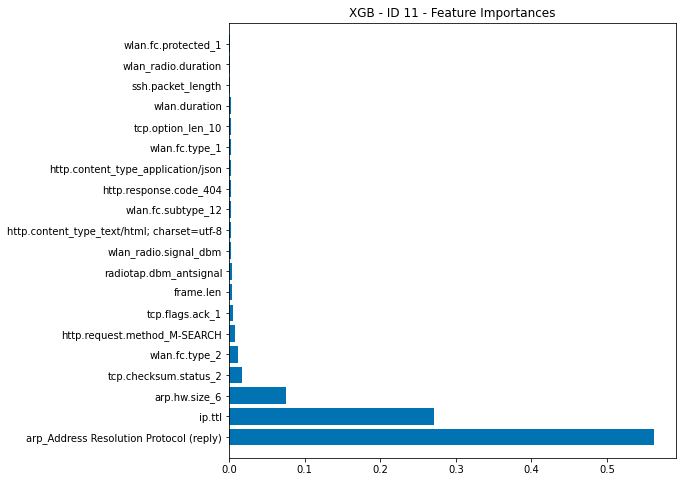
\includegraphics[width=\textwidth]{Appendices/Images/XGB/Model11/XGB_Model11_FI.png}
	\captionof*{figure}{XGBoost Model 11 - Feature Importance}
\end{center}


\clearpage
\section{Neural Networks}
\label{appx: Neural Networks}

\subsubsection{MLP Model 0 - Raw Metrics}
\begin{lstlisting}[escapechar=!]
!\textbf{S-CV Results}!


!\textbf{Final Test Results}!
Test AUC: 99.9858021736145
Weighted Test F1:  99.3620514961493
Weighted Test Precision:  99.38432657598928
Weighted Test Recall:  99.40703938402462
Test Accuracy:  99.40703938402462

!\textbf{Classification Report}!

			          precision    recall  f1-score   support

      Botnet       0.94      0.60      0.73     10236
     Malware       0.90      0.67      0.77     23686
      Normal       0.99      1.00      1.00   2743324
         SQL       1.00      0.08      0.15       473
        SSDP       1.00      1.00      1.00    989973
         SSH       0.89      0.46      0.61      2139
    WebSpoof       0.99      0.91      0.95     72920

    accuracy                           0.99   3842751
   macro avg       0.96      0.67      0.74   3842751
weighted avg       0.99      0.99      0.99   3842751
    
!\textbf{Confusion Matrix}!    
[[   6106      48    4054       0       0      22       6]
 [     40   15809    7810       0       0      27       0]
 [    299    1707 2740823       0      10      67     418]
 [      0       0     434      39       0       0       0]
 [      0       0      10       0  989963       0       0]
 [      2      13    1140       0       0     984       0]
 [     74       0    6603       0       2       0   66241]]

\end{lstlisting}


\subsubsection{MLP Model 1 - Raw Metrics}
\begin{lstlisting}[escapechar=!]
!\textbf{S-CV Results}!


!\textbf{Final Test Results}!

Test AUC: 0.9998605251312256
Weighted Test F1:  0.9934398041259884
Weighted Test Precision:  0.9935614162656269
Weighted Test Recall:  0.993817450050758
Test Accuracy:  0.993817450050758

!\textbf{Classification Report}!

			          precision    recall  f1-score   support

      Botnet       0.87      0.58      0.70     10236
     Malware       0.88      0.71      0.79     23686
      Normal       0.99      1.00      1.00   2743324
         SQL       1.00      0.38      0.55       473
        SSDP       1.00      1.00      1.00    989973
         SSH       0.91      0.45      0.60      2139
    WebSpoof       0.99      0.89      0.94     72920

    accuracy                           0.99   3842751
   macro avg       0.95      0.72      0.80   3842751
weighted avg       0.99      0.99      0.99   3842751
    
!\textbf{Confusion Matrix}!
    
[[   5977      36    4205       0       0      14       4]
 [    219   16928    6531       0       0       8       0]
 [    603    2233 2740011       0       9      74     394]
 [      2       5     282     181       0       3       0]
 [      0       0       9       0  989964       0       0]
 [      1      22    1151       0       0     965       0]
 [     30      12    7909       0       2       0   64967]]

\end{lstlisting}


\subsubsection{MLP Model 2 - Raw Metrics}
\begin{lstlisting}[escapechar=!]

!\textbf{Final Test Results}!

Test AUC:  0.9986337212130303
Weighted Test Precision:  0.9942064571755157
Weighted Test Recall:  0.9943597037043976
Weighted Test F1:  0.9939107235001085
Test Accuracy:  0.9943597037043976

!\textbf{Classification Report}!

			          precision    recall  f1-score   support

      Botnet       0.93      0.62      0.74     13648
     Malware       0.96      0.64      0.77     31581
      Normal       0.99      1.00      1.00   3657765
         SQL       1.00      0.13      0.23       631
        SSDP       1.00      1.00      1.00   1319964
         SSH       0.84      0.57      0.68      2852
    WebSpoof       1.00      0.91      0.95     97226

    accuracy                           0.99   5123667
   macro avg       0.96      0.70      0.77   5123667
weighted avg       0.99      0.99      0.99   5123667
    
!\textbf{Confusion Matrix}!
    
[[   8403     163    5018       0       0      26      38]
[     36   20332   11185       0       0      28       0]
[    550     770 3655857       0      12     258     318]
[      0       0     548      83       0       0       0]
[      0       0      12       0 1319952       0       0]
[     12       0    1222       0       0    1618       0]
[     33      16    8653       0       1       0   88523]]

\end{lstlisting}

\subsubsection{MLP Model 3 - Raw Metrics}
\begin{lstlisting}[escapechar=!]

!\textbf{Final Test Results}!

Test AUC: 0.9998477896054586
Weighted Test F1:  0.9939352564175636
Weighted Test Precision:  0.9943562023089472
Weighted Test Recall:  0.9944416762447676
Test Accuracy:  0.9944416762447676

!\textbf{Classification Report}!

			          precision    recall  f1-score   support

      Botnet       0.92      0.63      0.75     13648
     Malware       0.99      0.62      0.76     31581
      Normal       0.99      1.00      1.00   3657765
         SQL       1.00      0.15      0.25       631
        SSDP       1.00      1.00      1.00   1319964
         SSH       0.93      0.45      0.61      2852
    WebSpoof       1.00      0.92      0.95     97226

    accuracy                           0.99   5123667
   macro avg       0.98      0.68      0.76   5123667
weighted avg       0.99      0.99      0.99   5123667
    
!\textbf{Confusion Matrix}! 
   
[[   8644      40    4952       0       0       2      10]
 [    295   19427   11852       0       0       7       0]
 [    409     246 3656779       0       9      84     238]
 [      0       0     538      92       1       0       0]
 [      0       0      16       0 1319948       0       0]
 [      5       0    1569       0       0    1278       0]
 [     25       2    8178       0       1       0   89020]]

\end{lstlisting}


\subsubsection{MLP Model 4 - Raw Metrics}
\begin{lstlisting}[escapechar=!]
!\textbf{S-CV Results}!
Average AUC: 99.90
Average F1: 99.37
Average Precision: 99.40
Average Recall: 99.42
Average Accuracy: 99.42
CV Time 2007.377500295639 seconds

!\textbf{Final Test Results}!
Test AUC:  0.9993877331212752
Weighted Test F1:  0.9942475033645454
Weighted Test Precision:  0.9943763031781035
Weighted Test Recall:  0.994580131980469
Test Accuracy:  0.994580131980469

!\textbf{Classification Report}!
			           precision    recall  f1-score   support

      Botnet       0.94      0.61      0.74     17060
     Malware       0.89      0.72      0.80     39476
      Normal       0.99      1.00      1.00   4572206
         SQL       0.99      0.37      0.54       789
        SSDP       1.00      1.00      1.00   1649955
         SSH       0.83      0.48      0.60      3565
    WebSpoof       1.00      0.92      0.95    121533

    accuracy                           0.99   6404584
   macro avg       0.95      0.73      0.80   6404584
weighted avg       0.99      0.99      0.99   6404584
    
!\textbf{Confusion Matrix}!    
 [[  10357     139    6453       0       0     101      10]
 [    112   28556   10769       0       0      39       0]
 [    507    3351 4567732       2       8     205     401]
 [      0       0     495     294       0       0       0]
 [      0       0      10       0 1649945       0       0]
 [      0      28    1842       0       0    1695       0]
 [     34      11   10194       0       1       0  111293]]
\end{lstlisting}

\begin{figure}[H]
    \caption{MLP Model 4 - Loss Curves}
    \centering
    \begin{minipage}[b]{0.40\textwidth}
        \subcaptionbox{Fold 1}{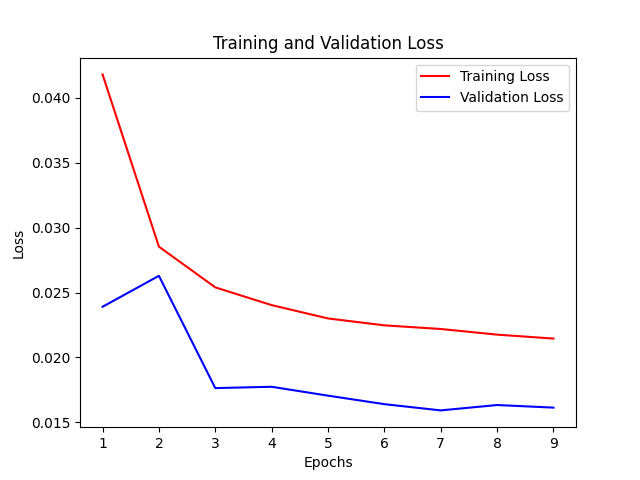
\includegraphics[width=\linewidth]{Appendices/Images/MLP/Model4/MLP_Fold_1_Loss.png}}
        \subcaptionbox{Fold 2}{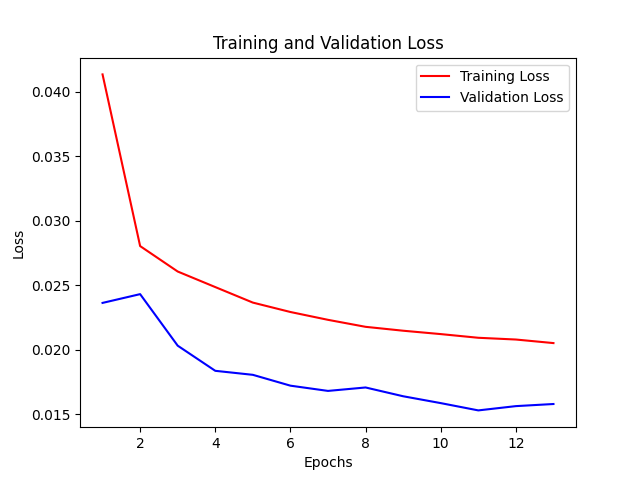
\includegraphics[width=\linewidth]{Appendices/Images/MLP/Model4/MLP_Fold_2_Loss.png}}
        \subcaptionbox{Fold 3}{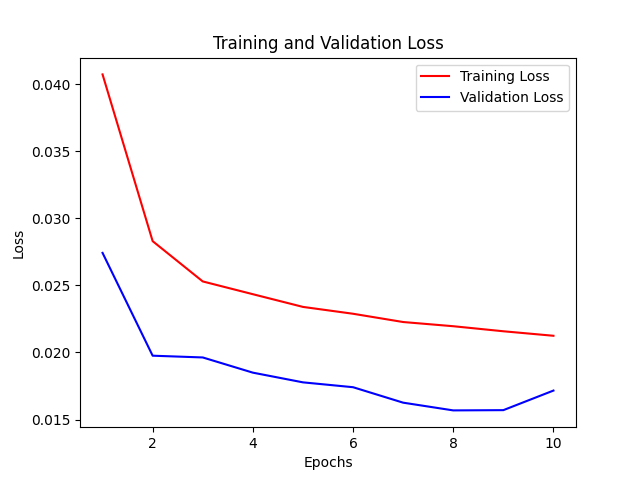
\includegraphics[width=\linewidth]{Appendices/Images/MLP/Model4/MLP_Fold_3_Loss.png}}
        \subcaptionbox{Fold 4}{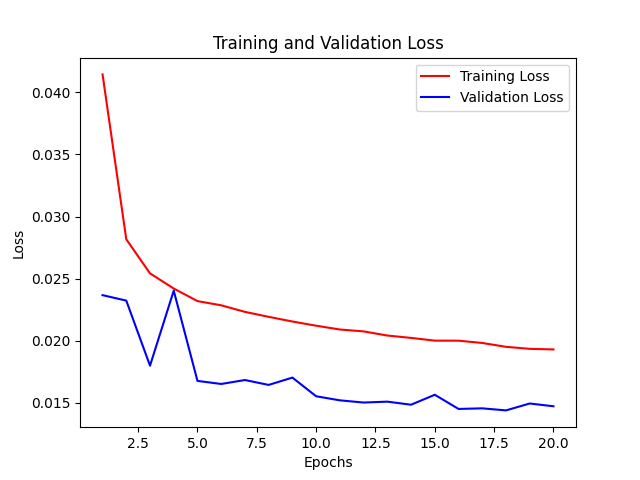
\includegraphics[width=\linewidth]{Appendices/Images/MLP/Model4/MLP_Fold_4_Loss.png}}
        \subcaptionbox{Fold 5}{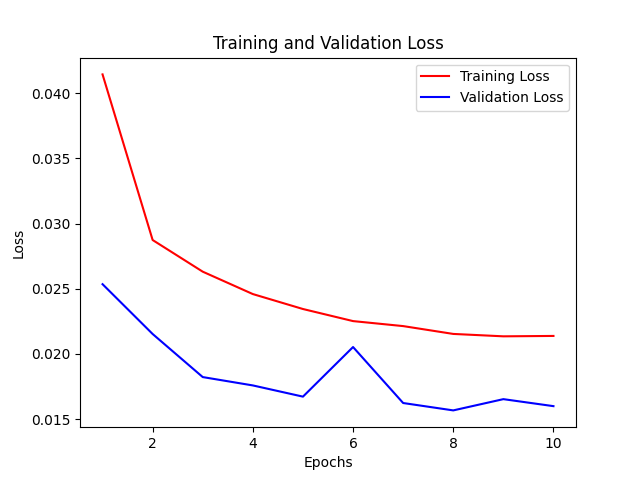
\includegraphics[width=\linewidth]{Appendices/Images/MLP/Model4/MLP_Fold_5_Loss.png}}
    \end{minipage}
    \hfill
    \begin{minipage}[b]{0.40\textwidth}
        \subcaptionbox{Fold 6}{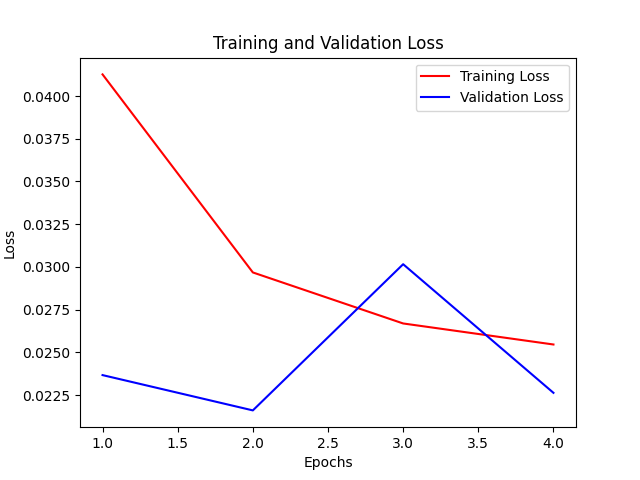
\includegraphics[width=\linewidth]{Appendices/Images/MLP/Model4/MLP_Fold_6_Loss.png}}
        \subcaptionbox{Fold 7}{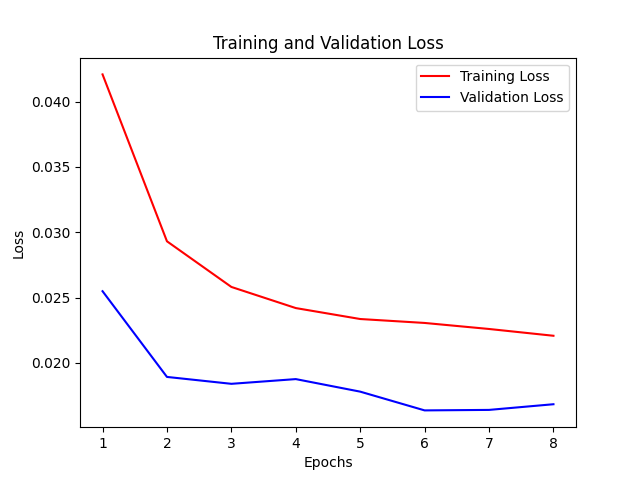
\includegraphics[width=\linewidth]{Appendices/Images/MLP/Model4/MLP_Fold_7_Loss.png}}
        \subcaptionbox{Fold 8}{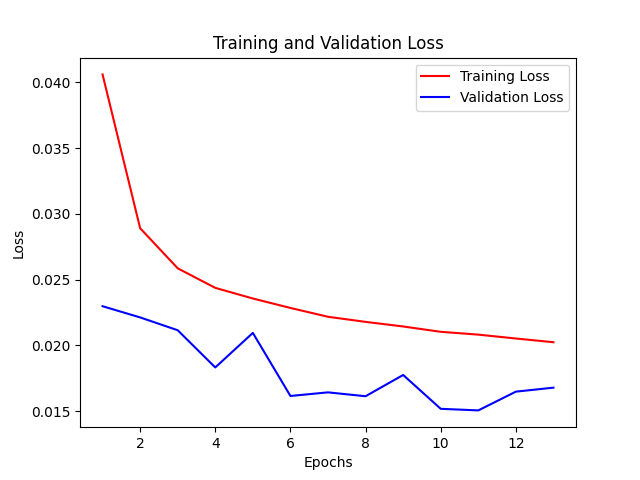
\includegraphics[width=\linewidth]{Appendices/Images/MLP/Model4/MLP_Fold_8_Loss.png}}
        \subcaptionbox{Fold 9}{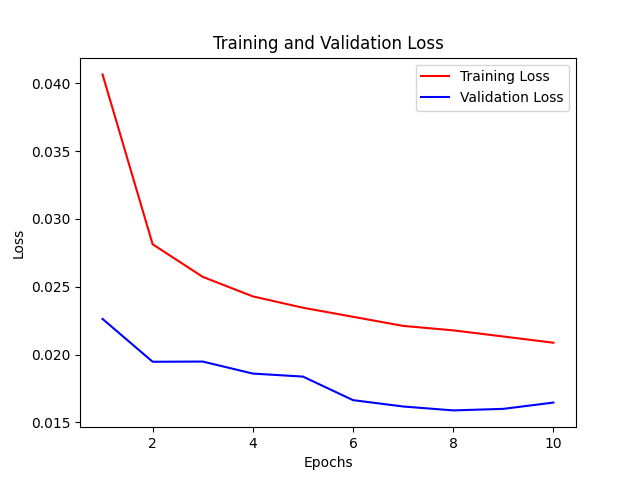
\includegraphics[width=\linewidth]{Appendices/Images/MLP/Model4/MLP_Fold_9_Loss.png}}
        \subcaptionbox{Fold 10}{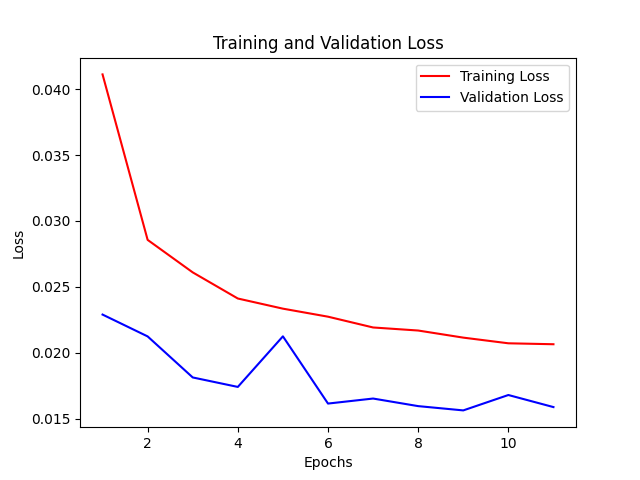
\includegraphics[width=\linewidth]{Appendices/Images/MLP/Model4/MLP_Fold_10_Loss.png}}
    \end{minipage}
\end{figure}

\subsubsection{MLP Model 5 - Raw Metrics}
\begin{lstlisting}[escapechar=!]
!\textbf{S-CV Results}!
AUC: 0.9840
F1: 0.9468
Precision: 0.9685
Recall: 0.9549
Accuracy: 0.9549
CV Time: 1892.0350830554962 seconds

!\textbf{Final Test Results}!
Test AUC: 0.9988450838388412
Weighted Test F1: 0.9935567670757577
Weighted Test Precision: 0.993714141198025
Weighted Test Recall: 0.9940441096564585
Test Accuracy: 0.9940441096564585

!\textbf{Classification Report}!

			           precision    recall  f1-score   support

      Botnet       0.87      0.54      0.66     17060
     Malware       0.90      0.64      0.75     39476
      Normal       0.99      1.00      1.00   4572206
         SQL       0.99      0.34      0.51       789
        SSDP       1.00      1.00      1.00   1649955
         SSH       0.80      0.47      0.59      3565
    WebSpoof       0.99      0.92      0.95    121533

    accuracy                           0.99   6404584
   macro avg       0.94      0.70      0.78   6404584
weighted avg       0.99      0.99      0.99   6404584
    
!\textbf{Confusion Matrix}!    
[[   9180    1338    6411       0       0     124       7]
[      9   25233   14198       0       0      36       0]
[   1206    1337 4568726       3      20     258     656]
[      0       0     513     270       2       4       0]
[      0       0      10       0 1649945       0       0]
[      0       1    1877       0       0    1687       0]
[    196       1    9935       0       3       0  111398]]

\end{lstlisting}


\subsubsection{MLP Model 6 - Raw Metrics}
\begin{lstlisting}[escapechar=!]
!\textbf{S-CV Results}!
AUC: 0.9979
F1: 0.9927
Precision: 0.9931
Recall: 0.9933
Accuracy: 0.9933
CV Time: 4323.574688911438 seconds

!\textbf{Final Test Results}!
Test AUC: 0.9979510725501038
Weighted Test F1: 0.9937794324941432
Weighted Test Precision: 0.9939653920793858
Weighted Test Recall: 0.9941811989662405
Test Accuracy: 0.9941811989662405

!\textbf{Classification Report}!
			           precision    recall  f1-score   support

      Botnet       0.96      0.52      0.68     17060
     Malware       0.83      0.72      0.77     39476
      Normal       0.99      1.00      1.00   4572206
         SQL       0.98      0.13      0.22       789
        SSDP       1.00      1.00      1.00   1649955
         SSH       0.91      0.47      0.62      3565
    WebSpoof       0.98      0.94      0.96    121533

    accuracy                           0.99   6404584
   macro avg       0.95      0.68      0.75   6404584
weighted avg       0.99      0.99      0.99   6404584
    
!\textbf{Confusion Matrix}!    
[[   8899     195    7823       0       0      17     126]
 [     43   28231   11177       0       0      25       0]
 [    244    4724 4564566       2      12     122    2536]
 [      0       0     689     100       0       0       0]
 [      0       0      10       0 1649945       0       0]
 [      0     519    1388       0       0    1658       0]
 [     62     237    7315       0       1       0  113918]]

\end{lstlisting}

\subsubsection{MLP Model 7 - Raw Metrics}
\begin{lstlisting}[escapechar=!]
!\textbf{S-CV Results}!
AUC: 99.72
F1: 99.23
Precision: 99.25
Recall: 99.31
Accuracy: 99.31
CV Time: 3009.0557339191437 seconds

!\textbf{Final Test Results}!
Test AUC: 99.8447719823538
Weighted Test F1: 99.28992200626915
Weighted Test Precision: 99.32770674412539
Weighted Test Recall: 99.35299466756935
Test Accuracy: 99.35299466756935

!\textbf{Classification Report}!
       		    precision    recall  f1-score   support
       		  
           0       0.86      0.55      0.67     17060
           1       0.95      0.60      0.74     39476
           2       0.99      1.00      1.00   4572206
           3       1.00      0.02      0.05       789
           4       1.00      1.00      1.00   1649955
           5       0.85      0.38      0.53      3565
           6       1.00      0.89      0.94    121533

    accuracy                           0.99   6404584
   macro avg       0.95      0.64      0.70   6404584
weighted avg       0.99      0.99      0.99   6404584
    
!\textbf{Confusion Matrix}!    
[[   9331      80    7565       0       0      78       6]
 [    725   23750   14955       0       0      46       0]
 [    787     882 4570078       0      15     116     328]
 [      4       0     766      19       0       0       0]
 [      0       0      10       0 1649945       0       0]
 [      4       0    2191       0       0    1370       0]
 [     56     236   12587       0       1       0  108653]]

\end{lstlisting}

\begin{center}
	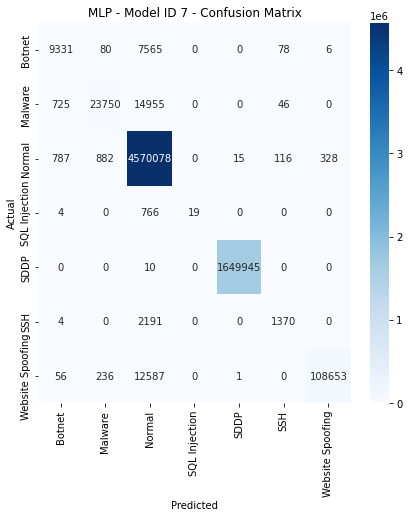
\includegraphics[width=\textwidth]{Appendices/Images/MLP/Model7/MLP_Model7_CM.png}
	\captionof*{figure}{MLP Model 7 - CM}
\end{center}


% ----------------------CODE -------------
\section{Model Code}
\label{appx: Model Code}

The following contains sections of the code relevant to creating the models. Only the 'best models' were included in this section to reduce repeating code and reduce the size of the appendices. The complete code for every model can be found in the code.zip and the full code base. 

\subsection{Data Cleaning}
\label{appx: Data Cleaning}
The following section contains the steps required to process the individual datasets for each class. 
\subsubsection*{Botnet}
\begin{lstlisting}[language=Python]
import pandas as pd
import re

# Define the columns to keep
cols_to_use = ['frame.len', 'radiotap.dbm_antsignal', 'radiotap.length', 'wlan.duration',
                   'wlan_radio.duration', 'wlan_radio.signal_dbm', 'radiotap.present.tsft',
                   'wlan.fc.type', 'wlan.fc.subtype', 'wlan.fc.ds', 'wlan.fc.frag',
                   'wlan.fc.moredata', 'wlan.fc.protected', 'wlan.fc.pwrmgt', 'wlan.fc.retry',
                   'wlan_radio.phy', 'udp.length', 'ip.ttl', 'arp', 'arp.proto.type',
                   'arp.hw.size', 'arp.proto.size', 'arp.hw.type', 'arp.opcode',
                   'tcp.analysis', 'tcp.analysis.retransmission', 'tcp.option_len',
                   'tcp.checksum.status', 'tcp.flags.ack', 'tcp.flags.fin', 'tcp.flags.push',
                   'tcp.flags.reset', 'tcp.flags.syn', 'dns', 'dns.count.queries', 'dns.count.answers',
                   'dns.resp.len', 'dns.resp.ttl', 'http.request.method', 'http.response.code',
                   'http.content_type', 'ssh.message_code', 'ssh.packet_length', 'nbns',
                   'nbss.length', 'nbss.type', 'ldap', 'smb2.cmd', 'smb.flags.response',
                   'smb.access.generic_read', 'smb.access.generic_write', 'smb.access.generic_execute','Label']

# Define the chunk size to read in each pass
batch_size = 1000000

combined_df = pd.DataFrame()

# Iterate through the file in batches
for chunk in pd.read_csv('botnet_reduced.csv', chunksize=batch_size, usecols=cols_to_use, low_memory=False):
    
    # Combine the processed chunk with previous chunks
    combined_df = pd.concat([combined_df, chunk])

# Drop all missing rows that contain only nan values
combined_df = combined_df.dropna(how='all')

# Drop all rows with missing values in Label Column
combined_df = combined_df.dropna(subset=['Label'])


# Fill NAs with zeros
# Change nan values to 0
combined_df = combined_df.fillna(0)

# Duplicate the df
df = combined_df.copy()

# Regex to keep only the first value e.g 
# -100-100-10 becomes -100,   123-456-1 becomes 123, -10-2 becomes-10, 81-63-63 becomes 81
def seperated_values(x):
    x = str(x)
    match = re.match(r'^(-?\d+).*$', x)
    if match:
        return match.group(1)
    else:
        return x
    
# Go through all columns and change separate values into just one value
for column in df.columns:
    df[column] = df[column].apply(seperated_values)
    print('Processing', column)
print('Done')


# Find Rows that contain values such as Oct-26, Oct-18, Feb-10 etc.. as these appear to be invalid and we will drop these rows.
regex = r"\b(?:\d{2}|(?:Jan|Feb|Mar|Apr|May|Jun|Jul|Aug|Sep|Oct|Nov|Dec))-(?:\d{2}|(?:Jan|Feb|Mar|Apr|May|Jun|Jul|Aug|Sep|Oct|Nov|Dec))\b"

# Use str.match method to apply the regex pattern to the column
mask = df['tcp.option_len'].astype(str).str.match(regex).fillna(False)
# Filter the dataframe
df = df[~mask]

# Use str.match method to apply the regex pattern to the column
mask = df['dns.resp.ttl'].astype(str).str.match(regex).fillna(False)
df = df[~mask]

# Use str.match method to apply the regex pattern to the column
mask = df['ip.ttl'].astype(str).str.match(regex).fillna(False)
df = df[~mask]

# Use str.match method to apply the regex pattern to the column
mask = df['smb2.cmd'].astype(str).str.match(regex).fillna(False)
df = df[~mask]

df.to_csv('botnet.csv', index=False)
\end{lstlisting}

\subsubsection*{Malware}
\begin{lstlisting}[language=Python]
import pandas as pd
import re

# Define the columns to keep
cols_to_use = ['frame.len', 'radiotap.dbm_antsignal', 'radiotap.length', 'wlan.duration',
                   'wlan_radio.duration', 'wlan_radio.signal_dbm', 'radiotap.present.tsft',
                   'wlan.fc.type', 'wlan.fc.subtype', 'wlan.fc.ds', 'wlan.fc.frag',
                   'wlan.fc.moredata', 'wlan.fc.protected', 'wlan.fc.pwrmgt', 'wlan.fc.retry',
                   'wlan_radio.phy', 'udp.length', 'ip.ttl', 'arp', 'arp.proto.type',
                   'arp.hw.size', 'arp.proto.size', 'arp.hw.type', 'arp.opcode',
                   'tcp.analysis', 'tcp.analysis.retransmission', 'tcp.option_len',
                   'tcp.checksum.status', 'tcp.flags.ack', 'tcp.flags.fin', 'tcp.flags.push',
                   'tcp.flags.reset', 'tcp.flags.syn', 'dns', 'dns.count.queries', 'dns.count.answers',
                   'dns.resp.len', 'dns.resp.ttl', 'http.request.method', 'http.response.code',
                   'http.content_type', 'ssh.message_code', 'ssh.packet_length', 'nbns',
                   'nbss.length', 'nbss.type', 'ldap', 'smb2.cmd', 'smb.flags.response',
                   'smb.access.generic_read', 'smb.access.generic_write', 'smb.access.generic_execute','Label']

# Define the chunk size to read in each pass
batch_size = 1000000

combined_df = pd.DataFrame()

# Iterate through the file in batches
for chunk in pd.read_csv('malware_reduced.csv', chunksize=batch_size, usecols=cols_to_use, low_memory=False):
    
    # Combine the processed chunk with previous chunks
    combined_df = pd.concat([combined_df, chunk])

# Drop all missing rows that contain only nan values
combined_df = combined_df.dropna(how='all')

# Drop all rows with missing values in Label Column
combined_df = combined_df.dropna(subset=['Label'])

# Fill NAs with zeros
# Change nan values to 0
combined_df = combined_df.fillna(0)

# Duplicate the dataframe
df = combined_df.copy()

# ## Seperate Hyphen Values

# Regex to keep only the first value e.g 
# -100-100-10 becomes -100,   123-456-1 becomes 123, -10-2 becomes-10, 81-63-63 becomes 81
def seperated_values(x):
    x = str(x)
    match = re.match(r'^(-?\d+).*$', x)
    if match:
        return match.group(1)
    else:
        return x

# Go through all columns and change seperate values into just one value
for column in df.columns:
    df[column] = df[column].apply(seperated_values)
    print('Processing', column)
print('Done')

df['Label'].value_counts()
df['tcp.option_len'].value_counts()
df['ip.ttl'].value_counts()
df['dns.resp.ttl'].value_counts()

# Find Rows that contain values such as Oct-26, Oct-18, Feb-10 etc.. as these appear to be invalid and we will drop these rows.
regex = r"\b(?:\d{2}|(?:Jan|Feb|Mar|Apr|May|Jun|Jul|Aug|Sep|Oct|Nov|Dec))-(?:\d{2}|(?:Jan|Feb|Mar|Apr|May|Jun|Jul|Aug|Sep|Oct|Nov|Dec))\b"

# ### tcp.option_len
# Use str.match method to apply the regex pattern to the column
mask = df['tcp.option_len'].astype(str).str.match(regex).fillna(False)
df = df[~mask] # Filter the dataframe
df['tcp.option_len'].value_counts()

# ### dns.resp.ttl
# Use str.match method to apply the regex pattern to the column
mask = df['dns.resp.ttl'].astype(str).str.match(regex).fillna(False)
df = df[~mask]
df['dns.resp.ttl'].value_counts()

# ### ip.ttl
# Use str.match method to apply the regex pattern to the column
mask = df['ip.ttl'].astype(str).str.match(regex).fillna(False)
df = df[~mask] # Filter the dataframe
df['ip.ttl'].value_counts()

# ### smb2.cmd
# Use str.match method to apply the regex pattern to the column
mask = df['smb2.cmd'].astype(str).str.match(regex).fillna(False)
df = df[~mask] # Filter the dataframe
df['smb2.cmd'].value_counts()

# ## Export to CSV
df.to_csv('malware.csv', index=False)	
\end{lstlisting}

\subsubsection*{SQL}
\begin{lstlisting}[language=Python]
import pandas as pd
import re

# Define the columns to keep
cols_to_use = ['frame.len', 'radiotap.dbm_antsignal', 'radiotap.length', 'wlan.duration',
                   'wlan_radio.duration', 'wlan_radio.signal_dbm', 'radiotap.present.tsft',
                   'wlan.fc.type', 'wlan.fc.subtype', 'wlan.fc.ds', 'wlan.fc.frag',
                   'wlan.fc.moredata', 'wlan.fc.protected', 'wlan.fc.pwrmgt', 'wlan.fc.retry',
                   'wlan_radio.phy', 'udp.length', 'ip.ttl', 'arp', 'arp.proto.type',
                   'arp.hw.size', 'arp.proto.size', 'arp.hw.type', 'arp.opcode',
                   'tcp.analysis', 'tcp.analysis.retransmission', 'tcp.option_len',
                   'tcp.checksum.status', 'tcp.flags.ack', 'tcp.flags.fin', 'tcp.flags.push',
                   'tcp.flags.reset', 'tcp.flags.syn', 'dns', 'dns.count.queries', 'dns.count.answers',
                   'dns.resp.len', 'dns.resp.ttl', 'http.request.method', 'http.response.code',
                   'http.content_type', 'ssh.message_code', 'ssh.packet_length', 'nbns',
                   'nbss.length', 'nbss.type', 'ldap', 'smb2.cmd', 'smb.flags.response',
                   'smb.access.generic_read', 'smb.access.generic_write', 'smb.access.generic_execute','Label']

# Define the chunk size to read in each pass
batch_size = 1000000

combined_df = pd.DataFrame()

# Iterate through the file in batches
for chunk in pd.read_csv('sql_reduce.csv', chunksize=batch_size, usecols=cols_to_use, low_memory=False):
    
    # Combine the processed chunk with previous chunks
    combined_df = pd.concat([combined_df, chunk])

combined_df.info()

# Check for missing values
combined_df.isna().sum()

# Drop all missing rows that contain only nan values
combined_df = combined_df.dropna(how='all')

# Drop all rows with missing values in Label Column
combined_df = combined_df.dropna(subset=['Label'])

# Fill NAs with zeros
# Change nan values to 0
combined_df = combined_df.fillna(0)

# Duplicate the dataframe
df = combined_df.copy()
df.info()

# ## Seperate Hyphen Values

# Regex to keep only the first value e.g 
# -100-100-10 becomes -100,   123-456-1 becomes 123, -10-2 becomes-10, 81-63-63 becomes 81
def seperated_values(x):
    x = str(x)
    match = re.match(r'^(-?\d+).*$', x)
    if match:
        return match.group(1)
    else:
        return x

# Go through all columns and change separate values into just one value
for column in df.columns:
    df[column] = df[column].apply(seperated_values)
    print('Processing', column)
print('Done')

df['Label'].value_counts()
df['tcp.option_len'].value_counts()
df['ip.ttl'].value_counts()
df['dns.resp.ttl'].value_counts()
# Find Rows that contain values such as Oct-26, Oct-18, Feb-10 etc.. as these appear to be invalid and we will drop these rows.
regex = r"\b(?:\d{2}|(?:Jan|Feb|Mar|Apr|May|Jun|Jul|Aug|Sep|Oct|Nov|Dec))-(?:\d{2}|(?:Jan|Feb|Mar|Apr|May|Jun|Jul|Aug|Sep|Oct|Nov|Dec))\b"

# ### tcp.option_len
# Use str.match method to apply the regex pattern to the column
mask = df['tcp.option_len'].astype(str).str.match(regex).fillna(False)
df = df[~mask]
df['tcp.option_len'].value_counts()

# ### dns.resp.ttl
# Use str.match method to apply the regex pattern to the column
mask = df['dns.resp.ttl'].astype(str).str.match(regex).fillna(False)
df = df[~mask]
df['dns.resp.ttl'].value_counts()

# ### ip.ttl
# Use str.match method to apply the regex pattern to the column
mask = df['ip.ttl'].astype(str).str.match(regex).fillna(False)
df = df[~mask]
df['ip.ttl'].value_counts()

# ### smb2.cmd
# Use str.match method to apply the regex pattern to the column
mask = df['smb2.cmd'].astype(str).str.match(regex).fillna(False)
df = df[~mask]
df['smb2.cmd'].value_counts()

# ## Export to CSV
df.to_csv('sql_reduced.csv', index=False)	
\end{lstlisting}


\subsubsection*{SSDP}
\begin{lstlisting}[language=Python]
import pandas as pd
import re
from sklearn.model_selection import train_test_split

# Define the columns to keep
cols_to_use = ['frame.len', 'radiotap.dbm_antsignal', 'radiotap.length', 'wlan.duration',
                   'wlan_radio.duration', 'wlan_radio.signal_dbm', 'radiotap.present.tsft',
                   'wlan.fc.type', 'wlan.fc.subtype', 'wlan.fc.ds', 'wlan.fc.frag',
                   'wlan.fc.moredata', 'wlan.fc.protected', 'wlan.fc.pwrmgt', 'wlan.fc.retry',
                   'wlan_radio.phy', 'udp.length', 'ip.ttl', 'arp', 'arp.proto.type',
                   'arp.hw.size', 'arp.proto.size', 'arp.hw.type', 'arp.opcode',
                   'tcp.analysis', 'tcp.analysis.retransmission', 'tcp.option_len',
                   'tcp.checksum.status', 'tcp.flags.ack', 'tcp.flags.fin', 'tcp.flags.push',
                   'tcp.flags.reset', 'tcp.flags.syn', 'dns', 'dns.count.queries', 'dns.count.answers',
                   'dns.resp.len', 'dns.resp.ttl', 'http.request.method', 'http.response.code',
                   'http.content_type', 'ssh.message_code', 'ssh.packet_length', 'nbns',
                   'nbss.length', 'nbss.type', 'ldap', 'smb2.cmd', 'smb.flags.response',
                   'smb.access.generic_read', 'smb.access.generic_write', 'smb.access.generic_execute','Label']

# Define the chunk size to read in each pass
batch_size = 1000000

combined_df = pd.DataFrame()

# Iterate through the file in batches
for chunk in pd.read_csv('ssdp_combined.csv', chunksize=batch_size, usecols=cols_to_use, low_memory=False):
    
    # Combine the processed chunk with previous chunks
    combined_df = pd.concat([combined_df, chunk])

combined_df.info()
combined_df.isna().sum()

# Drop all missing rows that contain only nan values
combined_df = combined_df.dropna(how='all')

# Drop all rows with missing values in Label Column
combined_df = combined_df.dropna(subset=['Label'])

combined_df = combined_df.fillna(0) # Change nan values to 0
df = combined_df.copy() # Duplicate the dataframe

df = df.reindex(columns=cols_to_use)

# ## Decimal To Int

# Convert any floats that contain no decimals into integer datatypes

# Define the column name to search for decimals
column_name = 'wlan.duration'
# Create a regular expression pattern to match numbers with decimals
decimal_pattern = r'\d+\.\d+'

# Count the number of matches in the specified column
decimal_count = 0
for value in df[column_name]:
    if isinstance(value, str) and re.search(decimal_pattern, value):
        decimal_count += 1

# Print the result
print(f"The number of rows with decimals in column '{column_name}' is {decimal_count}.")

df[['radiotap.length','ip.ttl']] = df[['radiotap.length', 'ip.ttl'[].astype(int)
#df['ip.ttl'] = df['ip.ttl'].astype(int)
#df['wlan.duration'] = df['wlan.duration'].astype(int)

# ## Seperate Hyphen Values

# Regex to keep only the first value e.g 
# -100-100-10 becomes -100,   123-456-1 becomes 123, -10-2 becomes-10, 81-63-63 becomes 81
def seperated_values(x):
    x = str(x)
    match = re.match(r'^(-?\d+).*$', x)
    if match:
        return match.group(1)
    else:
        return x

# Go through all columns and change seperate values into just one value
for column in df.columns:
    df[column] = df[column].apply(seperated_values)
    print('Processing', column)

df['tcp.option_len'].value_counts()

# Find Rows that contain values such as Oct-26, Oct-18, Feb-10 etc.. as these appear to be invalid and we will drop these rows.
#regex = r"\b(?:Jan|Feb|Mar|Apr|May|Jun|Jul|Aug|Sep|Oct|Nov|Dec)-\d{2}\b"
regex = r"\b(?:\d{2}|(?:Jan|Feb|Mar|Apr|May|Jun|Jul|Aug|Sep|Oct|Nov|Dec))-(?:\d{2}|(?:Jan|Feb|Mar|Apr|May|Jun|Jul|Aug|Sep|Oct|Nov|Dec))\b"

for index, row in df.iterrows():
    # If the value is a string and matches the regex
    if isinstance(row['tcp.option_len'], str) and re.search(regex, row['tcp.option_len']):
        #print(row['tcp.option_len'])
        df.drop(index, inplace=True) # Drop the value in place by its index

for index, row in df.iterrows():
    # If the value is a string and matches the regex
    if isinstance(row['ip.ttl'], str) and re.search(regex, row['ip.ttl']):
        df.drop(index, inplace=True) # Drop the value in place by its index

for index, row in df.iterrows():
    # If the value is a string and matches the regex
    if isinstance(row['dns.resp.ttl'], str) and re.search(regex, row['dns.resp.ttl']):
        df.drop(index, inplace=True) # Drop the value in place by its index

# Use str.match method to apply the regex pattern to the column
mask = df['tcp.option_len'].astype(str).str.match(regex).fillna(False)

# Filter the dataframe
df = df[~mask]

df['tcp.option_len'].value_counts()

# Use str.match method to apply the regex pattern to the column
mask = df['dns.resp.ttl'].astype(str).str.match(regex).fillna(False)

# Filter the dataframe
df = df[~mask]

df['dns.resp.ttl'].value_counts()

# Use str.match method to apply the regex pattern to the column
mask = df['ip.ttl'].astype(str).str.match(regex).fillna(False)

# Filter the dataframe
df = df[~mask]

df['ip.ttl'].value_counts()
df['Label'] = df['Label'].replace({'SDDP': 'SSDP'})

df.to_csv('sddp.csv', index=False)

# # Testing

combined_df.to_csv('ssdp_reduced.csv',  index=False)
batch_size = 1000000
combined_df = pd.DataFrame()

# Iterate through the file in batches
for chunk in pd.read_csv('ssdp_reduced.csv', chunksize=batch_size, low_memory=False):
    
    # Combine the processed chunk with previous chunks
    combined_df = pd.concat([combined_df, chunk])

combined_df.head()

combined_df['radiotap.dbm_antsignal'].value_counts()

processed_df = combined_df.copy()
processed_df['radiotap.dbm_antsignal'] = combined_df['radiotap.dbm_antsignal'].apply(seperated_values)
processed_df['dns.resp.ttl'] = combined_df['dns.resp.ttl'].apply(seperated_values)
processed_df['udp.length'] = combined_df['udp.length'].apply(seperated_values)
processed_df['ip.ttl'] = combined_df['ip.ttl'].apply(seperated_values)
processed_df['dns.count.answers'] = combined_df['dns.count.answers'].apply(seperated_values)
processed_df['nbss.length'] = combined_df['nbss.length'].apply(seperated_values)
processed_df['smb2.cmd'] = combined_df['smb2.cmd'].apply(seperated_values)
processed_df['ssh.packet_length'] = combined_df['ssh.packet_length'].apply(seperated_values)
processed_df['ssh.message_code'] = combined_df['ssh.message_code'].apply(seperated_values)
combined_df['ip.ttl'].value_counts()
processed_df['ip.ttl'].value_counts()

# Define the column name to search for decimals
column_name = 'ip.ttl'

# Create a regular expression pattern to match numbers with decimals
decimal_pattern = r'\d+\.\d+'

# Count the number of matches in the specified column
decimal_count = 0
for value in combined_df[column_name]:
    if isinstance(value, str) and re.search(decimal_pattern, value):
        print(value)
        decimal_count += 1

# Print the result
print(f"The number of rows with decimals in column '{column_name}' is {decimal_count}.")

def separated_values(x):
    # Convert x to a string and remove any leading/trailing whitespaces
    x = str(x).strip()
    # Use regex to check if x contains any non-digit character
    if re.search(r'\D', x):
        # x contains non-digit character, so return None to mark for removal
        return None
    else:
        # x contains only digits, so apply the original separated_values logic
        match = re.match(r'^(-?\d+).*$', x)
        if match:
            print(match.group(1))
            return match.group(1)
        else:
            return x

processed_df['ip.ttl'] = combined_df['ip.ttl'].apply(seperated_values)
#processed_df = processed_df.dropna()

# Change Data Types

processed_df['udp.length'] = processed_df['udp.length'].astype(float).astype(int)
processed_df.head()

# ### Subset of data
processed_df['Label'].value_counts()
processed_df.isna().sum()

#  Encode the target variable, 0 is Normal, 1 is SSH, 2 is SQL Injection
processed_df['Label'] = processed_df['Label'].map({'Normal': 0, 'SDDP': 1})

# Split the data into training and testing sets, preserving the class distribution
train_data, test_data, train_labels, test_labels = train_test_split(processed_df.drop('Label', axis=1), processed_df['Label'], test_size=0.5, stratify=processed_df['Label'])

train_data.value_counts()
# Combine the training data and labels
reduced_df = pd.concat([train_data, train_labels], axis=1)

# Export the subset of data to a CSV file
reduced_df.to_csv('ssdp_reduced.csv', index=False)	
\end{lstlisting}

\subsubsection*{SSH}
\begin{lstlisting}[language=Python]
import pandas as pd
import re

# Define the columns to keep
cols_to_use = ['frame.len', 'radiotap.dbm_antsignal', 'radiotap.length', 'wlan.duration',
                   'wlan_radio.duration', 'wlan_radio.signal_dbm', 'radiotap.present.tsft',
                   'wlan.fc.type', 'wlan.fc.subtype', 'wlan.fc.ds', 'wlan.fc.frag',
                   'wlan.fc.moredata', 'wlan.fc.protected', 'wlan.fc.pwrmgt', 'wlan.fc.retry',
                   'wlan_radio.phy', 'udp.length', 'ip.ttl', 'arp', 'arp.proto.type',
                   'arp.hw.size', 'arp.proto.size', 'arp.hw.type', 'arp.opcode',
                   'tcp.analysis', 'tcp.analysis.retransmission', 'tcp.option_len',
                   'tcp.checksum.status', 'tcp.flags.ack', 'tcp.flags.fin', 'tcp.flags.push',
                   'tcp.flags.reset', 'tcp.flags.syn', 'dns', 'dns.count.queries', 'dns.count.answers',
                   'dns.resp.len', 'dns.resp.ttl', 'http.request.method', 'http.response.code',
                   'http.content_type', 'ssh.message_code', 'ssh.packet_length', 'nbns',
                   'nbss.length', 'nbss.type', 'ldap', 'smb2.cmd', 'smb.flags.response',
                   'smb.access.generic_read', 'smb.access.generic_write', 'smb.access.generic_execute','Label']

# Define the chunk size to read in each pass
batch_size = 1000000

combined_df = pd.DataFrame()

# Iterate through the file in batches
for chunk in pd.read_csv('ssh_reduced.csv', chunksize=batch_size, usecols=cols_to_use, low_memory=False):
    
    # Combine the processed chunk with previous chunks
    combined_df = pd.concat([combined_df, chunk])

combined_df.info()

# Check for missing values
combined_df.isna().sum()

# Drop all missing rows that contain only nan values
combined_df = combined_df.dropna(how='all')

# Drop all rows with missing values in Label Column
combined_df = combined_df.dropna(subset=['Label'])

# Fill NAs with zeros
# Change nan values to 0
combined_df = combined_df.fillna(0)

# Duplicate the dataframe
df = combined_df.copy()

df.info()

# Regex to keep only the first value e.g 
# -100-100-10 becomes -100,   123-456-1 becomes 123, -10-2 becomes-10, 81-63-63 becomes 81
def seperated_values(x):
    x = str(x)
    match = re.match(r'^(-?\d+).*$', x)
    if match:
        return match.group(1)
    else:
        return x

# Go through all columns and change separate values into just one value
for column in df.columns:
    df[column] = df[column].apply(seperated_values)
    print('Processing', column)
print('Done')

df['Label'].value_counts()
df['tcp.option_len'].value_counts()
df['ip.ttl'].value_counts()
df['dns.resp.ttl'].value_counts()

# Find Rows that contain values such as Oct-26, Oct-18, Feb-10 etc.. as these appear to be invalid and we will drop these rows.
regex = r"\b(?:\d{2}|(?:Jan|Feb|Mar|Apr|May|Jun|Jul|Aug|Sep|Oct|Nov|Dec))-(?:\d{2}|(?:Jan|Feb|Mar|Apr|May|Jun|Jul|Aug|Sep|Oct|Nov|Dec))\b"

# ### tcp.option_len
# Use str.match method to apply the regex pattern to the column
mask = df['tcp.option_len'].astype(str).str.match(regex).fillna(False)
# Filter the dataframe
df = df[~mask]
df['tcp.option_len'].value_counts()

# ### dns.resp.ttl
# Use str.match method to apply the regex pattern to the column
mask = df['dns.resp.ttl'].astype(str).str.match(regex).fillna(False)
df = df[~mask]
df['dns.resp.ttl'].value_counts()


# ### ip.ttl
mask = df['ip.ttl'].astype(str).str.match(regex).fillna(False)
df = df[~mask]
df['ip.ttl'].value_counts()


# ### smb2.cmd
mask = df['smb2.cmd'].astype(str).str.match(regex).fillna(False)
df = df[~mask]
df['smb2.cmd'].value_counts()

# ## Export to CSV
df.to_csv('ssh.csv', index=False)	
\end{lstlisting}

\subsubsection*{Website Spoofing}
\begin{lstlisting}[language=Python]
import pandas as pd
import re

# Define the columns to keep
cols_to_use = ['frame.len', 'radiotap.dbm_antsignal', 'radiotap.length', 'wlan.duration',
                   'wlan_radio.duration', 'wlan_radio.signal_dbm', 'radiotap.present.tsft',
                   'wlan.fc.type', 'wlan.fc.subtype', 'wlan.fc.ds', 'wlan.fc.frag',
                   'wlan.fc.moredata', 'wlan.fc.protected', 'wlan.fc.pwrmgt', 'wlan.fc.retry',
                   'wlan_radio.phy', 'udp.length', 'ip.ttl', 'arp', 'arp.proto.type',
                   'arp.hw.size', 'arp.proto.size', 'arp.hw.type', 'arp.opcode',
                   'tcp.analysis', 'tcp.analysis.retransmission', 'tcp.option_len',
                   'tcp.checksum.status', 'tcp.flags.ack', 'tcp.flags.fin', 'tcp.flags.push',
                   'tcp.flags.reset', 'tcp.flags.syn', 'dns', 'dns.count.queries', 'dns.count.answers',
                   'dns.resp.len', 'dns.resp.ttl', 'http.request.method', 'http.response.code',
                   'http.content_type', 'ssh.message_code', 'ssh.packet_length', 'nbns',
                   'nbss.length', 'nbss.type', 'ldap', 'smb2.cmd', 'smb.flags.response',
                   'smb.access.generic_read', 'smb.access.generic_write', 'smb.access.generic_execute','Label']

# Define the chunk size to read in each pass
batch_size = 1000000

combined_df = pd.DataFrame()

# Iterate through the file in batches
for chunk in pd.read_csv('website_spoofing_reduced.csv', chunksize=batch_size, usecols=cols_to_use, low_memory=False):  
    # Combine the processed chunk with previous chunks
    combined_df = pd.concat([combined_df, chunk])

combined_df.info()
# Check for missing values
combined_df.isna().sum()

# Drop all missing rows that contain only nan values
combined_df = combined_df.dropna(how='all')
# Drop all rows with missing values in Label Column
combined_df = combined_df.dropna(subset=['Label'])

# Fill NAs with zeros
# Change nan values to 0
combined_df = combined_df.fillna(0)

# Duplicate the dataframe
df = combined_df.copy()
df.info()

# ## Decimal To Int

# Convert any floats that contain no decimals into integer datatypes

# ## Seperate Hyphen Values

# Regex to keep only the first value e.g 
# -100-100-10 becomes -100,   123-456-1 becomes 123, -10-2 becomes-10, 81-63-63 becomes 81
def seperated_values(x):
    x = str(x)
    match = re.match(r'^(-?\d+).*$', x)
    if match:
        return match.group(1)
    else:
        return x

# Go through all columns and change separate values into just one value
for column in df.columns:
    df[column] = df[column].apply(seperated_values)
    print('Processing', column)
df['Label'].value_counts()
df['tcp.option_len'].value_counts()
df['ip.ttl'].value_counts()
df['dns.resp.ttl'].value_counts()

# Find Rows that contain values such as Oct-26, Oct-18, Feb-10 etc.. as these appear to be invalid and we will drop these rows.
regex = r"\b(?:\d{2}|(?:Jan|Feb|Mar|Apr|May|Jun|Jul|Aug|Sep|Oct|Nov|Dec))-(?:\d{2}|(?:Jan|Feb|Mar|Apr|May|Jun|Jul|Aug|Sep|Oct|Nov|Dec))\b"
for index, row in df.iterrows():
    # If the value is a string and matches the regex
    if isinstance(row['tcp.option_len'], str) and re.search(regex, row['tcp.option_len']):
        #print(row['tcp.option_len'])
        df.drop(index, inplace=True) # Drop the value in place by its index

for index, row in df.iterrows():
    # If the value is a string and matches the regex
    if isinstance(row['ip.ttl'], str) and re.search(regex, row['ip.ttl']):
        df.drop(index, inplace=True) # Drop the value in place by its index

for index, row in df.iterrows():
    # If the value is a string and matches the regex
    if isinstance(row['dns.resp.ttl'], str) and re.search(regex, row['dns.resp.ttl']):
        df.drop(index, inplace=True) # Drop the value in place by its index

# ### tcp.option_len
# Use str.match method to apply the regex pattern to the column
mask = df['tcp.option_len'].astype(str).str.match(regex).fillna(False)

# Filter the dataframe
df = df[~mask]
df['tcp.option_len'].value_counts()

# ### dns.resp.ttl
mask = df['dns.resp.ttl'].astype(str).str.match(regex).fillna(False)
df = df[~mask]
df['dns.resp.ttl'].value_counts()

# ### ip.ttl
mask = df['ip.ttl'].astype(str).str.match(regex).fillna(False)
df = df[~mask]
df['ip.ttl'].value_counts()

# ## Export to CSV
df.to_csv('website_reduced.csv', index=False)	
\end{lstlisting}

\subsection{Data Import - Code}
\label{appx: Data Import - Code}
\begin{lstlisting}[language=Python]
import pandas as pd
from sklearn.model_selection import train_test_split
from sklearn.preprocessing import MinMaxScaler
from sklearn.preprocessing import LabelEncoder
import numpy as np

def load_data():
    chunk_size = 1000000
    dtype_opt = {
        'frame.len': 'int64',
        'radiotap.dbm_antsignal': 'int64',
        'radiotap.length': 'int64',
        'radiotap.present.tsft': 'int64',
        'wlan.duration': 'int64',
        'wlan.fc.ds': 'int64',
        'wlan.fc.frag': 'int64',
        'wlan.fc.moredata': 'int64',
        'wlan.fc.protected': 'int64',
        'wlan.fc.pwrmgt': 'int64',
        'wlan.fc.type': 'int64',
        'wlan.fc.retry': 'int64',
        'wlan.fc.subtype': 'int64',
        'wlan_radio.duration': 'int64',
        'wlan_radio.signal_dbm': 'int64',
        'wlan_radio.phy': 'int64',
        'arp': 'object',
        'arp.hw.type': 'object',
        'arp.proto.type': 'int64',
        'arp.hw.size': 'int64',
        'arp.proto.size': 'int64',
        'arp.opcode': 'int64',
        'ip.ttl': 'int64',
        'tcp.analysis': 'int64',
        'tcp.analysis.retransmission': 'int64',
        'tcp.checksum.status': 'int64',
        'tcp.flags.syn': 'int64',
        'tcp.flags.ack': 'int64',
        'tcp.flags.fin': 'int64',
        'tcp.flags.push': 'int64',
        'tcp.flags.reset': 'int64',
        'tcp.option_len': 'int64',
        'udp.length': 'int64',
        'nbns': 'object',
        'nbss.length': 'int64',
        'ldap': 'object',
        'smb2.cmd': 'int64',
        'dns': 'object',
        'dns.count.answers': 'int64',
        'dns.count.queries': 'int64',
        'dns.resp.ttl': 'int64',
        'http.content_type': 'object',
        'http.request.method': 'object',
        'http.response.code': 'int64',
        'ssh.message_code': 'int64',
        'ssh.packet_length': 'int64'
    }

    # Read the data
    print('Reading X...')
    X = pd.DataFrame()
    for chunk in pd.read_csv('/tf/notebooks/Notebooks/100%/X.csv', chunksize=chunk_size, usecols=dtype_opt.keys(), dtype=dtype_opt, low_memory=False):
        X = pd.concat([X, chunk])

    print('Reading y...')
    y = pd.DataFrame()
    for chunk in pd.read_csv('/tf/notebooks/Notebooks/100%/y.csv', chunksize=chunk_size, usecols=['Label'], dtype='object', low_memory=False):
        y = pd.concat([y, chunk])

    # Split the data into training and testing sets
    print('Splitting the data...')
    X_train, X_test, y_train, y_test = train_test_split(X, y, test_size=0.30, random_state=1234, stratify=y)
    del X, y

    # Scale the data
    print('Scaling the data...')
    scaler = MinMaxScaler()
    scale_cols = ['frame.len',
            'radiotap.dbm_antsignal', 
            'radiotap.length', 
            'wlan.duration', 
            'wlan_radio.duration', 
            'wlan_radio.signal_dbm',
            'ip.ttl', 
            'udp.length', 
            'nbss.length',
            'dns.count.answers', 
            'dns.count.queries',
            'dns.resp.ttl',
            'ssh.packet_length']

    X_train[scale_cols] = scaler.fit_transform(X_train[scale_cols])
    X_test[scale_cols] = scaler.transform(X_test[scale_cols])

    # Encode the labels
    print('Encoding X...')
    cols_to_encode = [col for col in X_train.columns if col not in scale_cols]
    X_all = pd.concat([X_train, X_test], axis=0)
    X_all_ohe = pd.get_dummies(X_all, columns=cols_to_encode, drop_first=True, dtype=np.uint8)
    X_train_ohe = X_all_ohe[:len(X_train)]
    X_test_ohe = X_all_ohe[len(X_train):]
    del X_all
    del X_all_ohe

    print('Label Encoding y...')
    le = LabelEncoder()
    y_train_encoded = le.fit_transform(y_train.values.ravel())
    y_test_encoded = le.transform(y_test.values.ravel())
    del y_train, y_test

    label_mapping = dict(zip(le.classes_, range(len(le.classes_))))
    print(label_mapping)

    return X_train_ohe, y_train_encoded, X_test_ohe, y_test_encoded	
\end{lstlisting}

\subsection{Data Import 2 - Code}
\label{appx: Data Import 2 - Code}
\begin{lstlisting}[language=Python]
import pandas as pd
from sklearn.model_selection import train_test_split
from sklearn.preprocessing import MinMaxScaler
from sklearn.preprocessing import LabelEncoder
import tensorflow as tf
from tensorflow.keras.utils import to_categorical
import numpy as np


def load_data():
    chunk_size = 1000000
    dtype_opt = {
        'frame.len': 'int64',
        'radiotap.dbm_antsignal': 'int64',
        'radiotap.length': 'int64',
        'radiotap.present.tsft': 'int64',
        'wlan.duration': 'int64',
        'wlan.fc.ds': 'int64',
        'wlan.fc.frag': 'int64',
        'wlan.fc.moredata': 'int64',
        'wlan.fc.protected': 'int64',
        'wlan.fc.pwrmgt': 'int64',
        'wlan.fc.type': 'int64',
        'wlan.fc.retry': 'int64',
        'wlan.fc.subtype': 'int64',
        'wlan_radio.duration': 'int64',
        'wlan_radio.signal_dbm': 'int64',
        'wlan_radio.phy': 'int64',
        'arp': 'object',
        'arp.hw.type': 'object',
        'arp.proto.type': 'int64',
        'arp.hw.size': 'int64',
        'arp.proto.size': 'int64',
        'arp.opcode': 'int64',
        'ip.ttl': 'int64',
        'tcp.analysis': 'int64',
        'tcp.analysis.retransmission': 'int64',
        'tcp.checksum.status': 'int64',
        'tcp.flags.syn': 'int64',
        'tcp.flags.ack': 'int64',
        'tcp.flags.fin': 'int64',
        'tcp.flags.push': 'int64',
        'tcp.flags.reset': 'int64',
        'tcp.option_len': 'int64',
        'udp.length': 'int64',
        'nbns': 'object',
        'nbss.length': 'int64',
        'ldap': 'object',
        'smb2.cmd': 'int64',
        'dns': 'object',
        'dns.count.answers': 'int64',
        'dns.count.queries': 'int64',
        'dns.resp.ttl': 'int64',
        'http.content_type': 'object',
        'http.request.method': 'object',
        'http.response.code': 'int64',
        'ssh.message_code': 'int64',
        'ssh.packet_length': 'int64'
    }

    # Read the data
    print('Reading X...')
    X = pd.DataFrame()
    for chunk in pd.read_csv('/Users/u2054584/Documents/ml-project/Datasets/combined/100%/X.csv', chunksize=chunk_size, usecols=dtype_opt.keys(), dtype=dtype_opt, low_memory=False):
        X = pd.concat([X, chunk])

    print('Reading y...')
    y = pd.DataFrame()
    for chunk in pd.read_csv('/Users/u2054584/Documents/ml-project/Datasets/combined/100%/y.csv', chunksize=chunk_size, usecols=['Label'], dtype='object', low_memory=False):
        y = pd.concat([y, chunk])

    # Split the data into training and testing sets
    print('Splitting the data...')
    X_train, X_test, y_train, y_test = train_test_split(X, y, test_size=0.30, random_state=1234, stratify=y)
    del X, y

    # Scale the data
    print('Scaling the data...')
    scaler = MinMaxScaler()
    scale_cols = [
        'frame.len',
        'radiotap.dbm_antsignal', 
        'radiotap.length', 
        'wlan.duration', 
        'wlan_radio.duration', 
        'wlan_radio.signal_dbm',
        'ip.ttl', 
        'udp.length', 
        'nbss.length',
        'dns.count.answers', 
        'dns.count.queries',
        'dns.resp.ttl',
        'ssh.packet_length']

    X_train[scale_cols] = scaler.fit_transform(X_train[scale_cols])
    X_test[scale_cols] = scaler.transform(X_test[scale_cols])

    # Encode the labels
    print('Encoding X...')
    cols_to_encode = [col for col in X_train.columns if col not in scale_cols]
    X_all = pd.concat([X_train, X_test], axis=0)
    X_all_ohe = pd.get_dummies(X_all, columns=cols_to_encode, drop_first=True, dtype=np.uint8)
    X_train_ohe = X_all_ohe[:len(X_train)]
    X_test_ohe = X_all_ohe[len(X_train):]
    del X_all
    del X_all_ohe

    print('Label Encoding y...')
    le = LabelEncoder()
    y_train_encoded = le.fit_transform(y_train.values.ravel())
    y_test_encoded = le.transform(y_test.values.ravel())
    y_train_ohe = to_categorical(y_train_encoded)
    y_test_ohe = to_categorical(y_test_encoded)
    del y_train, y_test

    return X_train_ohe, y_train_ohe, y_train_encoded, X_test_ohe, y_test_ohe, y_test_encoded	
\end{lstlisting}

\subsection{RF Model 1 - Code}
\label{appx: RF Model 1 - Code}
\begin{lstlisting}[language=Python]
# Create the model

start_time = time.time()

# Set up stratified k-fold CV
n_splits = 10
skf = StratifiedKFold(n_splits=n_splits, shuffle=True, random_state=1234)

auc_list = []
f1_list = []
precision_list = []
recall_list = []
accuracy_list = []

# Iterate over each fold
for fold_index, (train_index, val_index) in enumerate(skf.split(X_train_ohe, y_train_encoded)):

    fold_time = time.time()
    print(f'Fold {fold_index+1}')

    # Split the data into training and validation sets for this fold
    X_train_fold, X_val_fold = X_train_ohe.iloc[train_index], X_train_ohe.iloc[val_index]
    y_train_fold, y_val_fold = y_train_encoded[train_index], y_train_encoded[val_index]

    rf = RandomForestClassifier(random_state=1234, n_jobs=-1, verbose=1)
    rf.fit(X_train_fold, y_train_fold)
    
    # Make predictions on the validation set
    y_pred_fold = rf.predict(X_val_fold)
    y_pred_proba = rf.predict_proba(X_val_fold)
    
    # Compute evaluation metrics for this fold
    auc = roc_auc_score(y_val_fold, y_pred_proba, multi_class='ovr', average='weighted')
    f1 = f1_score(y_val_fold, y_pred_fold, average='weighted')
    precision = precision_score(y_val_fold, y_pred_fold, average='weighted')
    recall = recall_score(y_val_fold, y_pred_fold, average='weighted')
    accuracy = accuracy_score(y_val_fold, y_pred_fold)
    
    # Append the evaluation metrics to the lists
    auc_list.append(auc)
    f1_list.append(f1)
    precision_list.append(precision)
    recall_list.append(recall)
    accuracy_list.append(accuracy)
    
    # Print the evaluation metrics for this fold
    print(f"Fold {fold_index+1}: AUC = {auc:.4f}, F1 = {f1:.4f}, Precision = {precision:.4f}, Recall = {recall:.4f}, Accuracy = {accuracy:.4f}")

    print("Fold Time: ", time.time() - fold_time, " seconds")

# Compute the average of the evaluation metrics across all folds
auc_mean = np.mean(auc_list)
f1_mean = np.mean(f1_list)
precision_mean = np.mean(precision_list)
recall_mean = np.mean(recall_list)
accuracy_mean = np.mean(accuracy_list)

# Print the average of the evaluation metrics across all folds
print(f"\nMean AUC = {auc_mean:.4f}, Mean F1 = {f1_mean:.4f}, Mean Precision = {precision_mean:.4f}, Mean Recall = {recall_mean:.4f}, Mean Accuracy = {accuracy_mean:.4f}")

end_time = time.time()
print('Time for Training', end_time - start_time,  ' seconds')

print('\n Creating Final Model with Full Training Data....')

rf = RandomForestClassifier(random_state=1234, n_jobs=-1, verbose=2)
rf.fit(X_train_ohe, y_train_encoded)

# Evaluate the model
print('Evaluating...')

rf_y_pred = rf.predict(X_test_ohe)
rf_pred_proba = rf.predict_proba(X_test_ohe)

print('Weighted AUC: ', roc_auc_score(y_test_encoded, rf_y_pred, multi_class='ovr', average='weighted'))
print('Weighted Precision: ', precision_score(y_test_encoded, rf_y_pred, average='weighted'))
print('Weighted Recall: ', recall_score(y_test_encoded, rf_y_pred, average='weighted'))
print('Weighted F1: ', f1_score(y_test_encoded, rf_y_pred, average='weighted'))
print('Accuracy: ', accuracy_score(y_test_encoded, rf_y_pred))


report = classification_report(y_test_encoded, rf_y_pred)
print(report)

confusion = confusion_matrix(y_test_encoded, rf_y_pred)
print('Confusion Matrix\n')
print(confusion)

# Plot the confusion matrix

labels = ['Botnet', 'Malware', 'Normal', 'SQL Injection', 'SSDP', 'SSH', 'Website Spoofing' ]
plt.figure(figsize=(10,10))
sns.heatmap(confusion, annot=True, fmt='d', cmap='Blues', xticklabels=labels, yticklabels=labels)
plt.title('RF - Stock 100% - Confusion Matrix')
plt.xlabel('Predicted')
plt.ylabel('Actual')
plt.savefig('cm.png')

plt.figure(figsize=(15,15))
feat_importance = pd.Series(rf.feature_importances_, index=X_train_ohe.columns)
feat_importance.nlargest(20).plot(kind='barh')
plt.savefig('feature_imp.png')

filename = 'rf.joblib'
joblib.dump(rf, filename)
\end{lstlisting}


\subsection{XGBoost Model 10 - Code} 
\label{appx: XGB Model 10 - Code}

\begin{lstlisting}[language=Python]
print('Training...')

start_time = time.time()
xgb = XGBClassifier(tree_method='gpu_hist', gpu_id=0, 
                    eval_metric='merror', early_stopping_rounds=10, 
                    subsample=0.9, n_estimators=200, min_child_weight=3, 
                    max_depth=9, learning_rate=0.3, gamma=0, colsample_bytree=0.7, verbose=1)

skf = StratifiedKFold(n_splits=10, shuffle=True, random_state=1234)

aucs = []
f1s = []
precisions = []
recalls = []
accuracies = []

for train_index, test_index in skf.split(X_train_ohe, y_train_encoded):
    start_time = time.time()

    print('Training Fold....')

    X_train_fold, X_test_fold = X_train_ohe.iloc[train_index], X_train_ohe.iloc[test_index]
    y_train_fold, y_test_fold = y_train_encoded[train_index], y_train_encoded[test_index]
    
    xgb.fit(X_train_fold, y_train_fold, eval_set=[(X_test_fold, y_test_fold)], verbose=False)
    
    y_pred = xgb.predict(X_test_fold)
    y_pred_proba = xgb.predict_proba(X_test_fold)
    
    # Calculate and store the weighted metrics
    aucs.append(roc_auc_score(y_test_fold, y_pred_proba, multi_class='ovr', average='weighted'))
    f1s.append(f1_score(y_test_fold, y_pred, average='weighted'))
    precisions.append(precision_score(y_test_fold, y_pred, average='weighted'))
    recalls.append(recall_score(y_test_fold, y_pred, average='weighted'))
    accuracies.append(accuracy_score(y_test_fold, y_pred))
    
    print('Fold Metrics: ', "AUC: ", aucs[-1], "F1-score: ", f1s[-1], "Precision: ", precisions[-1], "Recall: ", recalls[-1], "Accuracy: ", accuracies[-1], "\n")
    elapsed_time = time.time() - start_time
    print(f'Time taken for fold: {elapsed_time:.2f} seconds')

# Calculate the average metrics
avg_auc = np.mean(aucs)
avg_f1 = np.mean(f1s)
avg_precision = np.mean(precisions)
avg_recall = np.mean(recalls)
avg_accuracy = np.mean(accuracies)

print("Average AUC:", avg_auc)
print("Average F1-score:", avg_f1)
print("Average Precision:", avg_precision)
print("Average Recall:", avg_recall)
print("Average Accuracy:", avg_accuracy)
elapsed_time = time.time() - start_time
print(f'Time taken for CV training: {elapsed_time:.2f} seconds')


# Train a final model on the entire training dataset and then evaluate its performance on the test set:
print('Training on entire training dataset...')
start_time = time.time()
eval_set = [(X_test_ohe, y_test_encoded)]
xgb.fit(X_train_ohe, y_train_encoded, eval_set=eval_set, verbose=True)
elapsed_time = time.time() - start_time
print(f'Time taken for final evaluation training: {elapsed_time:.2f} seconds')

print('Evaluating on test set...')

y_pred = xgb.predict(X_test_ohe)
predictions = [round(value) for value in y_pred]

# evaluate predictions

print('Test ROC AUC: ', roc_auc_score(y_test_encoded, xgb.predict_proba(X_test_ohe), multi_class='ovr'))
print('Test Precision: ', precision_score(y_test_encoded, y_pred, average='weighted'))
print('Test Recall: ', recall_score(y_test_encoded, y_pred, average='weighted'))
print('Test F1: ', f1_score(y_test_encoded, y_pred, average='weighted'))
print("Test Accuracy: ", accuracy_score(y_test_encoded, y_pred))

report = classification_report(y_test_encoded, y_pred)
print(report)

confusion = confusion_matrix(y_test_encoded, y_pred)
print('Confusion Matrix\n')
print(confusion)

# Plot the confusion matrix

labels = ['Botnet', 'Malware', 'Normal', 'SQL Injection', 'SSDP', 'SSH', 'Website Spoofing' ]
plt.figure(figsize=(10,10))
sns.heatmap(confusion, annot=True, fmt='d', cmap='Blues', xticklabels=labels, yticklabels=labels)
plt.title('Confusion Matrix')
plt.xlabel('Predicted')
plt.ylabel('Actual')
plt.savefig('cm.png')

filename = 'xgb.joblib'
joblib.dump(xgb, filename)
\end{lstlisting}

\subsection{MLP Model 4 - Code}
\label{appx: MLP Model 4 - Code}
\begin{lstlisting}[language=Python]
#  Train the model
print('Training...')

# Stratified K-Fold CV

# Define the number of folds
k_folds = 10

skf = StratifiedKFold(n_splits=k_folds, shuffle=True, random_state=1234)

# Define lists to store the evaluation metrics for each fold
auc_scores = []
precision_scores = []
recall_scores = []
f1_scores = []
accuracy_scores = []

# Record how long it took to train
start_time = time.time()

for fold_index, (train_index, val_index) in enumerate(skf.split(X_train_ohe, y_train_encoded)):
    plt.figure()
    print('\n---------Fold', fold_index+1, '-------')
    X_train_fold, X_val_fold = X_train_ohe.iloc[train_index], X_train_ohe.iloc[val_index]
    y_train_fold, y_val_fold = y_train_ohe[train_index], y_train_ohe[val_index]
    
    # Reset column names of X_train_ohe
    X_train_fold.columns = X_train_ohe.columns
    
    # Create the MLP
    model = Sequential()
    input_shape = (X_train_fold.shape[1],)
    early_stopping = EarlyStopping(monitor='val_loss', patience=2)

    model.add(Dense(units=128, activation='relu', kernel_initializer=he_uniform(), input_shape=input_shape))
    model.add(BatchNormalization())
    model.add(Dropout(0.2))
    
    model.add(Dense(units=64, activation='relu', kernel_initializer=he_uniform()))
    model.add(BatchNormalization())
    model.add(Dropout(0.2))
    
    model.add(Dense(units=32, activation='relu', kernel_initializer=he_uniform()))
    model.add(BatchNormalization())
    model.add(Dropout(0.2))
    
    model.add(Dense(units=y_train_ohe.shape[1], activation='softmax'))

    # Compile the model 
    model.compile(optimizer=Adam(learning_rate=0.001), loss='categorical_crossentropy', metrics=[AUC()])
    
    # Train the model
    start_time = time.time()
    history = model.fit(X_train_fold, y_train_fold, validation_data=(X_val_fold, y_val_fold), callbacks=[early_stopping], batch_size=200, epochs=20)
    end_time = time.time()
    
    print('Time to train fold:', end_time - start_time)
    
    # Predict on the test set and calculate metrics
    y_pred = np.argmax(model.predict(X_test_ohe), axis=1)
    y_pred_ohe = to_categorical(y_pred)
    
    auc = roc_auc_score(y_test_ohe, model.predict(X_test_ohe), multi_class='ovr')
    accuracy = accuracy_score(y_test_encoded, y_pred)
    precision = precision_score(y_test_encoded, y_pred, average='weighted')
    recall = recall_score(y_test_encoded, y_pred, average='weighted')
    f1 = f1_score(y_test_encoded, y_pred, average='weighted')
    
    print("Fold %d - AUC: %.4f, Accuracy: %.4f, Precision: %.4f, Recall: %.4f, F1: %.4f" % (fold_index+1, auc, accuracy, precision, recall, f1))
    
    # Save the metrics for this fold
    auc_scores.append(auc)
    accuracy_scores.append(accuracy)
    precision_scores.append(precision)
    recall_scores.append(recall)
    f1_scores.append(f1)

    train_loss = history.history['loss']
    val_loss = history.history['val_loss']
    epochs = range(1, len(train_loss) + 1)

    plt.plot(epochs, train_loss, 'r', label='Training Loss')
    plt.plot(epochs, val_loss, 'b', label='Validation Loss')
    plt.title('Training and Validation Loss')
    plt.xlabel('Num of Epochs')
    plt.ylabel('Loss')
    plt.legend()
    plt.savefig('MLP_Fold_' + str(fold_index+1) + '_Loss.png')
    
    del history
    K.clear_session() # Clear the keras session

# Calculate the average metrics for all folds
print("Average Metrics - AUC: %.4f, Accuracy: %.4f, Precision: %.4f, Recall: %.4f, F1: %.4f" % (np.mean(auc_scores), np.mean(accuracy_scores), np.mean(precision_scores), np.mean(recall_scores), np.mean(f1_scores)))

end_time = time.time()

#  Print the time it took to train
print('Time for CV:', end_time - start_time,  ' seconds')


print('\n Creating Final Model with Full Training Data....')

# Train the model on the entire training set
del model
plt.figure()
model = Sequential()
input_shape = (X_train_fold.shape[1],)
early_stopping = EarlyStopping(monitor='val_loss', patience=2)

model.add(Dense(units=128, activation='relu', kernel_initializer=he_uniform(), input_shape=input_shape))
model.add(BatchNormalization())
model.add(Dropout(0.2))

model.add(Dense(units=64, activation='relu', kernel_initializer=he_uniform()))
model.add(BatchNormalization())
model.add(Dropout(0.2))

model.add(Dense(units=32, activation='relu', kernel_initializer=he_uniform()))
model.add(BatchNormalization())
model.add(Dropout(0.2))

model.add(Dense(units=y_train_ohe.shape[1], activation='softmax'))

# Compile the model
model.compile(optimizer=Adam(learning_rate=0.001), loss='categorical_crossentropy', metrics=[AUC()])

# Train the model
history = model.fit(X_train_ohe, y_train_ohe, batch_size=200, callbacks=[early_stopping], epochs=20)

plt.plot(history.history['loss'])
plt.title('Training Loss vs Epoch')
plt.xlabel('Epoch')
plt.ylabel('Loss')
plt.savefig('MLP_Training_Loss.png')

print('\n Evaluating on test set...')

test_loss, test_auc = model.evaluate(X_test_ohe, y_test_ohe)

y_pred = model.predict(X_test_ohe)
y_pred_classes = np.argmax(y_pred, axis=1)
y_pred = np.argmax(y_pred, axis=1)
y_test_encoded = np.argmax(y_test_ohe, axis=1)

# Save the trained model
print('Saving Model...')
model.save('MLP.h5')

print('Weighted Test Accuracy: ', accuracy_score(y_test_encoded, y_pred))
print('Weighted Test Precision: ', precision_score(y_test_encoded, y_pred, average='weighted'))
print('Weighted Test Recall: ', recall_score(y_test_encoded, y_pred, average='weighted'))
print('Weighted Test AUC: ', roc_auc_score(y_test_ohe, y_pred, multi_class='ovr'))
print('Weighted Test F1: ', f1_score(y_test_encoded, y_pred, average='weighted'))

print('Confusion Matrix: \n', confusion_matrix(y_test_encoded, y_pred))
print('\nClassification Report: \n', classification_report(y_test_encoded, y_pred))
\end{lstlisting}

\end{appendices}


